\section{代码}

\begin{PythonCode}\label{例1}
	\begin{Verbatim}[commandchars=\\\{\}]
\PY{c+c1}{\PYZsh{} 导入操作系统库}
\PY{k+kn}{import} \PY{n+nn}{os}
\PY{c+c1}{\PYZsh{} 更改工作目录}
\PY{n}{os}\PY{o}{.}\PY{n}{chdir}\PY{p}{(}\PY{l+s+sa}{r}\PY{l+s+s2}{\PYZdq{}}\PY{l+s+s2}{D:}\PY{l+s+s2}{\PYZbs{}}\PY{l+s+s2}{softwares}\PY{l+s+s2}{\PYZbs{}}\PY{l+s+s2}{applied statistics}\PY{l+s+s2}{\PYZbs{}}\PY{l+s+s2}{pythoncodelearning}\PY{l+s+s2}{\PYZbs{}}\PY{l+s+s2}{chap6}\PY{l+s+s2}{\PYZbs{}}\PY{l+s+s2}{sourcecode}\PY{l+s+s2}{\PYZdq{}}\PY{p}{)}
\PY{c+c1}{\PYZsh{} 导入基础计算库}
\PY{k+kn}{import} \PY{n+nn}{numpy} \PY{k}{as} \PY{n+nn}{np}
\PY{c+c1}{\PYZsh{} 导入绘图库}
\PY{k+kn}{import} \PY{n+nn}{matplotlib}\PY{n+nn}{.}\PY{n+nn}{pyplot} \PY{k}{as} \PY{n+nn}{plt}
\PY{c+c1}{\PYZsh{} 导入bagging回归器}
\PY{k+kn}{from} \PY{n+nn}{sklearn}\PY{n+nn}{.}\PY{n+nn}{ensemble} \PY{k+kn}{import} \PY{n}{BaggingRegressor}
\PY{c+c1}{\PYZsh{} 导入决策树回归}
\PY{k+kn}{from} \PY{n+nn}{sklearn}\PY{n+nn}{.}\PY{n+nn}{tree} \PY{k+kn}{import} \PY{n}{DecisionTreeRegressor}
\PY{c+c1}{\PYZsh{} 导入绘图库中的字体管理包}
\PY{k+kn}{from} \PY{n+nn}{matplotlib} \PY{k+kn}{import} \PY{n}{font\PYZus{}manager}
\PY{c+c1}{\PYZsh{} 实现中文字符正常显示}
\PY{n}{font} \PY{o}{=} \PY{n}{font\PYZus{}manager}\PY{o}{.}\PY{n}{FontProperties}\PY{p}{(}\PY{n}{fname}\PY{o}{=}\PY{l+s+sa}{r}\PY{l+s+s2}{\PYZdq{}}\PY{l+s+s2}{C:}\PY{l+s+s2}{\PYZbs{}}\PY{l+s+s2}{Windows}\PY{l+s+s2}{\PYZbs{}}\PY{l+s+s2}{Fonts}\PY{l+s+s2}{\PYZbs{}}\PY{l+s+s2}{SimKai.ttf}\PY{l+s+s2}{\PYZdq{}}\PY{p}{)}
\PY{c+c1}{\PYZsh{} 使用seaborn风格绘图}
\PY{n}{plt}\PY{o}{.}\PY{n}{style}\PY{o}{.}\PY{n}{use}\PY{p}{(}\PY{l+s+s2}{\PYZdq{}}\PY{l+s+s2}{seaborn\PYZhy{}v0\PYZus{}8}\PY{l+s+s2}{\PYZdq{}}\PY{p}{)}
\PY{c+c1}{\PYZsh{} 计算期望的迭代次数}
\PY{n}{n\PYZus{}repeat} \PY{o}{=} \PY{l+m+mi}{50}
\PY{c+c1}{\PYZsh{} 训练集样本量}
\PY{n}{n\PYZus{}train} \PY{o}{=} \PY{l+m+mi}{50}
\PY{c+c1}{\PYZsh{} 测试集样本量}
\PY{n}{n\PYZus{}test} \PY{o}{=} \PY{l+m+mi}{1000}
\PY{c+c1}{\PYZsh{} 标准差}
\PY{n}{noise} \PY{o}{=} \PY{l+m+mf}{0.1}
\PY{n}{np}\PY{o}{.}\PY{n}{random}\PY{o}{.}\PY{n}{seed}\PY{p}{(}\PY{l+m+mi}{0}\PY{p}{)}
\PY{c+c1}{\PYZsh{} 构造模型}
\PY{n}{estimators} \PY{o}{=} \PY{p}{[}
    \PY{p}{(}\PY{l+s+s2}{\PYZdq{}}\PY{l+s+s2}{Tree}\PY{l+s+s2}{\PYZdq{}}\PY{p}{,} \PY{n}{DecisionTreeRegressor}\PY{p}{(}\PY{p}{)}\PY{p}{)}\PY{p}{,}
    \PY{p}{(}\PY{l+s+s2}{\PYZdq{}}\PY{l+s+s2}{Bagging(Tree)}\PY{l+s+s2}{\PYZdq{}}\PY{p}{,} \PY{n}{BaggingRegressor}\PY{p}{(}\PY{n}{DecisionTreeRegressor}\PY{p}{(}\PY{p}{)}\PY{p}{)}\PY{p}{)}\PY{p}{,}
\PY{p}{]}
\PY{c+c1}{\PYZsh{} 回归器的长度}
\PY{n}{n\PYZus{}estimators} \PY{o}{=} \PY{n+nb}{len}\PY{p}{(}\PY{n}{estimators}\PY{p}{)}
\PY{c+c1}{\PYZsh{} 生成x数据}
\PY{k}{def} \PY{n+nf}{f}\PY{p}{(}\PY{n}{x}\PY{p}{)}\PY{p}{:}
    \PY{n}{x} \PY{o}{=} \PY{n}{x}\PY{o}{.}\PY{n}{ravel}\PY{p}{(}\PY{p}{)}
    \PY{k}{return} \PY{n}{np}\PY{o}{.}\PY{n}{exp}\PY{p}{(}\PY{o}{\PYZhy{}}\PY{p}{(}\PY{n}{x}\PY{o}{*}\PY{o}{*}\PY{l+m+mi}{2}\PY{p}{)}\PY{p}{)} \PY{o}{+} \PY{l+m+mf}{1.5} \PY{o}{*} \PY{n}{np}\PY{o}{.}\PY{n}{exp}\PY{p}{(}\PY{o}{\PYZhy{}}\PY{p}{(}\PY{p}{(}\PY{n}{x} \PY{o}{\PYZhy{}} \PY{l+m+mi}{2}\PY{p}{)} \PY{o}{*}\PY{o}{*} \PY{l+m+mi}{2}\PY{p}{)}\PY{p}{)}
\PY{c+c1}{\PYZsh{} 生成XY数据}
\PY{k}{def} \PY{n+nf}{generate}\PY{p}{(}\PY{n}{n\PYZus{}samples}\PY{p}{,} \PY{n}{noise}\PY{p}{,} \PY{n}{n\PYZus{}repeat}\PY{o}{=}\PY{l+m+mi}{1}\PY{p}{)}\PY{p}{:}
    \PY{n}{X} \PY{o}{=} \PY{n}{np}\PY{o}{.}\PY{n}{random}\PY{o}{.}\PY{n}{rand}\PY{p}{(}\PY{n}{n\PYZus{}samples}\PY{p}{)} \PY{o}{*} \PY{l+m+mi}{10} \PY{o}{\PYZhy{}} \PY{l+m+mi}{5}
    \PY{n}{X} \PY{o}{=} \PY{n}{np}\PY{o}{.}\PY{n}{sort}\PY{p}{(}\PY{n}{X}\PY{p}{)}
    \PY{k}{if} \PY{n}{n\PYZus{}repeat} \PY{o}{==} \PY{l+m+mi}{1}\PY{p}{:}
        \PY{n}{y} \PY{o}{=} \PY{n}{f}\PY{p}{(}\PY{n}{X}\PY{p}{)} \PY{o}{+} \PY{n}{np}\PY{o}{.}\PY{n}{random}\PY{o}{.}\PY{n}{normal}\PY{p}{(}\PY{l+m+mf}{0.0}\PY{p}{,} \PY{n}{noise}\PY{p}{,} \PY{n}{n\PYZus{}samples}\PY{p}{)}
    \PY{k}{else}\PY{p}{:}
        \PY{n}{y} \PY{o}{=} \PY{n}{np}\PY{o}{.}\PY{n}{zeros}\PY{p}{(}\PY{p}{(}\PY{n}{n\PYZus{}samples}\PY{p}{,} \PY{n}{n\PYZus{}repeat}\PY{p}{)}\PY{p}{)}

        \PY{k}{for} \PY{n}{i} \PY{o+ow}{in} \PY{n+nb}{range}\PY{p}{(}\PY{n}{n\PYZus{}repeat}\PY{p}{)}\PY{p}{:}
            \PY{n}{y}\PY{p}{[}\PY{p}{:}\PY{p}{,} \PY{n}{i}\PY{p}{]} \PY{o}{=} \PY{n}{f}\PY{p}{(}\PY{n}{X}\PY{p}{)} \PY{o}{+} \PY{n}{np}\PY{o}{.}\PY{n}{random}\PY{o}{.}\PY{n}{normal}\PY{p}{(}\PY{l+m+mf}{0.0}\PY{p}{,} \PY{n}{noise}\PY{p}{,} \PY{n}{n\PYZus{}samples}\PY{p}{)}
    \PY{n}{X} \PY{o}{=} \PY{n}{X}\PY{o}{.}\PY{n}{reshape}\PY{p}{(}\PY{p}{(}\PY{n}{n\PYZus{}samples}\PY{p}{,} \PY{l+m+mi}{1}\PY{p}{)}\PY{p}{)}
    \PY{k}{return} \PY{n}{X}\PY{p}{,} \PY{n}{y}
\PY{c+c1}{\PYZsh{} 训练集列表}
\PY{n}{X\PYZus{}train} \PY{o}{=} \PY{p}{[}\PY{p}{]}
\PY{n}{y\PYZus{}train} \PY{o}{=} \PY{p}{[}\PY{p}{]}
\PY{c+c1}{\PYZsh{} 多个训练集}
\PY{k}{for} \PY{n}{i} \PY{o+ow}{in} \PY{n+nb}{range}\PY{p}{(}\PY{n}{n\PYZus{}repeat}\PY{p}{)}\PY{p}{:}
    \PY{n}{X}\PY{p}{,} \PY{n}{y} \PY{o}{=} \PY{n}{generate}\PY{p}{(}\PY{n}{n\PYZus{}samples}\PY{o}{=}\PY{n}{n\PYZus{}train}\PY{p}{,} \PY{n}{noise}\PY{o}{=}\PY{n}{noise}\PY{p}{)}
    \PY{n}{X\PYZus{}train}\PY{o}{.}\PY{n}{append}\PY{p}{(}\PY{n}{X}\PY{p}{)}
    \PY{n}{y\PYZus{}train}\PY{o}{.}\PY{n}{append}\PY{p}{(}\PY{n}{y}\PY{p}{)}
\PY{c+c1}{\PYZsh{} 生成一个测试集}
\PY{n}{X\PYZus{}test}\PY{p}{,} \PY{n}{y\PYZus{}test} \PY{o}{=} \PY{n}{generate}\PY{p}{(}\PY{n}{n\PYZus{}samples}\PY{o}{=}\PY{n}{n\PYZus{}test}\PY{p}{,} \PY{n}{noise}\PY{o}{=}\PY{n}{noise}\PY{p}{,} \PY{n}{n\PYZus{}repeat}\PY{o}{=}\PY{n}{n\PYZus{}repeat}\PY{p}{)}
\PY{c+c1}{\PYZsh{} 开始绘图}
\PY{n}{fig}\PY{p}{,} \PY{n}{axs} \PY{o}{=} \PY{n}{plt}\PY{o}{.}\PY{n}{subplots}\PY{p}{(}\PY{l+m+mi}{2}\PY{p}{,} \PY{l+m+mi}{2}\PY{p}{,} \PY{n}{figsize}\PY{o}{=}\PY{p}{(}\PY{l+m+mi}{10}\PY{p}{,} \PY{l+m+mi}{8}\PY{p}{)}\PY{p}{,} \PY{n}{tight\PYZus{}layout}\PY{o}{=}\PY{k+kc}{True}\PY{p}{)}
\PY{k}{for} \PY{n}{n}\PY{p}{,} \PY{p}{(}\PY{n}{name}\PY{p}{,} \PY{n}{estimator}\PY{p}{)} \PY{o+ow}{in} \PY{n+nb}{enumerate}\PY{p}{(}\PY{n}{estimators}\PY{p}{)}\PY{p}{:}
    \PY{c+c1}{\PYZsh{} 初始化预测值}
    \PY{n}{y\PYZus{}predict} \PY{o}{=} \PY{n}{np}\PY{o}{.}\PY{n}{zeros}\PY{p}{(}\PY{p}{(}\PY{n}{n\PYZus{}test}\PY{p}{,} \PY{n}{n\PYZus{}repeat}\PY{p}{)}\PY{p}{)}
    \PY{k}{for} \PY{n}{i} \PY{o+ow}{in} \PY{n+nb}{range}\PY{p}{(}\PY{n}{n\PYZus{}repeat}\PY{p}{)}\PY{p}{:}
        \PY{c+c1}{\PYZsh{} 模型拟合}
        \PY{n}{estimator}\PY{o}{.}\PY{n}{fit}\PY{p}{(}\PY{n}{X\PYZus{}train}\PY{p}{[}\PY{n}{i}\PY{p}{]}\PY{p}{,} \PY{n}{y\PYZus{}train}\PY{p}{[}\PY{n}{i}\PY{p}{]}\PY{p}{)}
        \PY{c+c1}{\PYZsh{} 模型预测}
        \PY{n}{y\PYZus{}predict}\PY{p}{[}\PY{p}{:}\PY{p}{,} \PY{n}{i}\PY{p}{]} \PY{o}{=} \PY{n}{estimator}\PY{o}{.}\PY{n}{predict}\PY{p}{(}\PY{n}{X\PYZus{}test}\PY{p}{)}
    \PY{c+c1}{\PYZsh{} 误差分解,初始化误差值}
    \PY{n}{y\PYZus{}error} \PY{o}{=} \PY{n}{np}\PY{o}{.}\PY{n}{zeros}\PY{p}{(}\PY{n}{n\PYZus{}test}\PY{p}{)}
    \PY{k}{for} \PY{n}{i} \PY{o+ow}{in} \PY{n+nb}{range}\PY{p}{(}\PY{n}{n\PYZus{}repeat}\PY{p}{)}\PY{p}{:}
        \PY{k}{for} \PY{n}{j} \PY{o+ow}{in} \PY{n+nb}{range}\PY{p}{(}\PY{n}{n\PYZus{}repeat}\PY{p}{)}\PY{p}{:}
            \PY{c+c1}{\PYZsh{} 计算预测值和真实值之间的误差}
            \PY{n}{y\PYZus{}error} \PY{o}{+}\PY{o}{=} \PY{p}{(}\PY{n}{y\PYZus{}test}\PY{p}{[}\PY{p}{:}\PY{p}{,} \PY{n}{j}\PY{p}{]} \PY{o}{\PYZhy{}} \PY{n}{y\PYZus{}predict}\PY{p}{[}\PY{p}{:}\PY{p}{,} \PY{n}{i}\PY{p}{]}\PY{p}{)} \PY{o}{*}\PY{o}{*} \PY{l+m+mi}{2}
    \PY{c+c1}{\PYZsh{} rescale一下}
    \PY{n}{y\PYZus{}error} \PY{o}{/}\PY{o}{=} \PY{n}{n\PYZus{}repeat} \PY{o}{*} \PY{n}{n\PYZus{}repeat}
    \PY{c+c1}{\PYZsh{} test数据集的噪声,方差}
    \PY{n}{y\PYZus{}noise} \PY{o}{=} \PY{n}{np}\PY{o}{.}\PY{n}{var}\PY{p}{(}\PY{n}{y\PYZus{}test}\PY{p}{,} \PY{n}{axis}\PY{o}{=}\PY{l+m+mi}{1}\PY{p}{)}
    \PY{c+c1}{\PYZsh{} 偏差平方和}
    \PY{n}{y\PYZus{}bias} \PY{o}{=} \PY{p}{(}\PY{n}{f}\PY{p}{(}\PY{n}{X\PYZus{}test}\PY{p}{)} \PY{o}{\PYZhy{}} \PY{n}{np}\PY{o}{.}\PY{n}{mean}\PY{p}{(}\PY{n}{y\PYZus{}predict}\PY{p}{,} \PY{n}{axis}\PY{o}{=}\PY{l+m+mi}{1}\PY{p}{)}\PY{p}{)} \PY{o}{*}\PY{o}{*} \PY{l+m+mi}{2}
    \PY{c+c1}{\PYZsh{} 预测值的方差}
    \PY{n}{y\PYZus{}var} \PY{o}{=} \PY{n}{np}\PY{o}{.}\PY{n}{var}\PY{p}{(}\PY{n}{y\PYZus{}predict}\PY{p}{,} \PY{n}{axis}\PY{o}{=}\PY{l+m+mi}{1}\PY{p}{)}
    \PY{n+nb}{print}\PY{p}{(}
        \PY{l+s+s2}{\PYZdq{}}\PY{l+s+si}{\PYZob{}0\PYZcb{}}\PY{l+s+s2}{: }\PY{l+s+si}{\PYZob{}1:.4f\PYZcb{}}\PY{l+s+s2}{ (error) = }\PY{l+s+si}{\PYZob{}2:.4f\PYZcb{}}\PY{l+s+s2}{ (bias\PYZca{}2) }\PY{l+s+s2}{\PYZdq{}}
        \PY{l+s+s2}{\PYZdq{}}\PY{l+s+s2}{ + }\PY{l+s+si}{\PYZob{}3:.4f\PYZcb{}}\PY{l+s+s2}{ (var) + }\PY{l+s+si}{\PYZob{}4:.4f\PYZcb{}}\PY{l+s+s2}{ (noise)}\PY{l+s+s2}{\PYZdq{}}\PY{o}{.}\PY{n}{format}\PY{p}{(}
            \PY{n}{name}\PY{p}{,} \PY{n}{np}\PY{o}{.}\PY{n}{mean}\PY{p}{(}\PY{n}{y\PYZus{}error}\PY{p}{)}\PY{p}{,} \PY{n}{np}\PY{o}{.}\PY{n}{mean}\PY{p}{(}\PY{n}{y\PYZus{}bias}\PY{p}{)}\PY{p}{,} 
            \PY{n}{np}\PY{o}{.}\PY{n}{mean}\PY{p}{(}\PY{n}{y\PYZus{}var}\PY{p}{)}\PY{p}{,} \PY{n}{np}\PY{o}{.}\PY{n}{mean}\PY{p}{(}\PY{n}{y\PYZus{}noise}\PY{p}{)}
        \PY{p}{)}
    \PY{p}{)}
    \PY{c+c1}{\PYZsh{} Plot figures}
    \PY{n}{ax1}\PY{o}{=}\PY{n}{axs}\PY{o}{.}\PY{n}{flatten}\PY{p}{(}\PY{p}{)}\PY{p}{[}\PY{n}{n}\PY{p}{]}
    \PY{c+c1}{\PYZsh{} 绘制测试集的真实值,无噪声}
    \PY{n}{ax1}\PY{o}{.}\PY{n}{plot}\PY{p}{(}\PY{n}{X\PYZus{}test}\PY{p}{,} \PY{n}{f}\PY{p}{(}\PY{n}{X\PYZus{}test}\PY{p}{)}\PY{p}{,} \PY{l+s+s2}{\PYZdq{}}\PY{l+s+s2}{b}\PY{l+s+s2}{\PYZdq{}}\PY{p}{,} \PY{n}{label}\PY{o}{=}\PY{l+s+s2}{\PYZdq{}}\PY{l+s+s2}{\PYZdl{}f(x)\PYZdl{}}\PY{l+s+s2}{\PYZdq{}}\PY{p}{)}
    \PY{c+c1}{\PYZsh{} 绘制训练集散点图,有噪声}
    \PY{n}{ax1}\PY{o}{.}\PY{n}{plot}\PY{p}{(}\PY{n}{X\PYZus{}train}\PY{p}{[}\PY{l+m+mi}{0}\PY{p}{]}\PY{p}{,} \PY{n}{y\PYZus{}train}\PY{p}{[}\PY{l+m+mi}{0}\PY{p}{]}\PY{p}{,} \PY{l+s+s2}{\PYZdq{}}\PY{l+s+s2}{.b}\PY{l+s+s2}{\PYZdq{}}\PY{p}{,} \PY{n}{label}\PY{o}{=}\PY{l+s+s2}{\PYZdq{}}\PY{l+s+s2}{LS \PYZti{} \PYZdl{}y = f(x)+noise\PYZdl{}}\PY{l+s+s2}{\PYZdq{}}\PY{p}{)}

    \PY{k}{for} \PY{n}{i} \PY{o+ow}{in} \PY{n+nb}{range}\PY{p}{(}\PY{n}{n\PYZus{}repeat}\PY{p}{)}\PY{p}{:}
        \PY{k}{if} \PY{n}{i} \PY{o}{==} \PY{l+m+mi}{0}\PY{p}{:}
            \PY{c+c1}{\PYZsh{} 测试集上的预测值}
            \PY{n}{ax1}\PY{o}{.}\PY{n}{plot}\PY{p}{(}\PY{n}{X\PYZus{}test}\PY{p}{,} \PY{n}{y\PYZus{}predict}\PY{p}{[}\PY{p}{:}\PY{p}{,} \PY{n}{i}\PY{p}{]}\PY{p}{,} \PY{l+s+s2}{\PYZdq{}}\PY{l+s+s2}{r}\PY{l+s+s2}{\PYZdq{}}\PY{p}{,} \PY{n}{label}\PY{o}{=}\PY{l+s+sa}{r}\PY{l+s+s2}{\PYZdq{}}\PY{l+s+s2}{\PYZdl{}}\PY{l+s+s2}{\PYZbs{}}\PY{l+s+s2}{\PYZca{}y(x)\PYZdl{}}\PY{l+s+s2}{\PYZdq{}}\PY{p}{)}
        \PY{k}{else}\PY{p}{:}
            \PY{c+c1}{\PYZsh{} 测试集上的预测值}
            \PY{n}{ax1}\PY{o}{.}\PY{n}{plot}\PY{p}{(}\PY{n}{X\PYZus{}test}\PY{p}{,} \PY{n}{y\PYZus{}predict}\PY{p}{[}\PY{p}{:}\PY{p}{,} \PY{n}{i}\PY{p}{]}\PY{p}{,} \PY{l+s+s2}{\PYZdq{}}\PY{l+s+s2}{r}\PY{l+s+s2}{\PYZdq{}}\PY{p}{,} \PY{n}{alpha}\PY{o}{=}\PY{l+m+mf}{0.05}\PY{p}{)}
    \PY{c+c1}{\PYZsh{} 测试集上的预测值的均值}
    \PY{n}{ax1}\PY{o}{.}\PY{n}{plot}\PY{p}{(}\PY{n}{X\PYZus{}test}\PY{p}{,} \PY{n}{np}\PY{o}{.}\PY{n}{mean}\PY{p}{(}\PY{n}{y\PYZus{}predict}\PY{p}{,} \PY{n}{axis}\PY{o}{=}\PY{l+m+mi}{1}\PY{p}{)}\PY{p}{,} \PY{l+s+s2}{\PYZdq{}}\PY{l+s+s2}{c}\PY{l+s+s2}{\PYZdq{}}\PY{p}{,} \PY{n}{label}\PY{o}{=}\PY{l+s+sa}{r}\PY{l+s+s2}{\PYZdq{}}\PY{l+s+s2}{\PYZdl{}}\PY{l+s+s2}{\PYZbs{}}\PY{l+s+s2}{mathbb}\PY{l+s+si}{\PYZob{}E\PYZcb{}}\PY{l+s+s2}{\PYZus{}}\PY{l+s+si}{\PYZob{}LS\PYZcb{}}\PY{l+s+s2}{ }\PY{l+s+s2}{\PYZbs{}}\PY{l+s+s2}{\PYZca{}y(x)\PYZdl{}}\PY{l+s+s2}{\PYZdq{}}\PY{p}{)}
    \PY{n}{ax1}\PY{o}{.}\PY{n}{set\PYZus{}xlim}\PY{p}{(}\PY{p}{[}\PY{o}{\PYZhy{}}\PY{l+m+mi}{5}\PY{p}{,} \PY{l+m+mi}{5}\PY{p}{]}\PY{p}{)}
    \PY{n}{ax1}\PY{o}{.}\PY{n}{set\PYZus{}title}\PY{p}{(}\PY{n}{name}\PY{p}{)}
    \PY{k}{if} \PY{n}{n} \PY{o}{==} \PY{n}{n\PYZus{}estimators} \PY{o}{\PYZhy{}} \PY{l+m+mi}{1}\PY{p}{:}
        \PY{n}{ax1}\PY{o}{.}\PY{n}{legend}\PY{p}{(}\PY{n}{loc}\PY{o}{=}\PY{p}{(}\PY{l+m+mf}{1.1}\PY{p}{,} \PY{l+m+mf}{0.5}\PY{p}{)}\PY{p}{)}

    \PY{n}{ax2} \PY{o}{=} \PY{n}{axs}\PY{o}{.}\PY{n}{flatten}\PY{p}{(}\PY{p}{)}\PY{p}{[}\PY{n}{n\PYZus{}estimators} \PY{o}{+} \PY{n}{n}\PY{p}{]}
    \PY{c+c1}{\PYZsh{} 测试集上的误差,偏差,方差,噪声}
    \PY{n}{ax2}\PY{o}{.}\PY{n}{plot}\PY{p}{(}\PY{n}{X\PYZus{}test}\PY{p}{,} \PY{n}{y\PYZus{}error}\PY{p}{,} \PY{l+s+s2}{\PYZdq{}}\PY{l+s+s2}{r}\PY{l+s+s2}{\PYZdq{}}\PY{p}{,} \PY{n}{label}\PY{o}{=}\PY{l+s+s2}{\PYZdq{}}\PY{l+s+s2}{\PYZdl{}error(x)\PYZdl{}}\PY{l+s+s2}{\PYZdq{}}\PY{p}{)}
    \PY{n}{ax2}\PY{o}{.}\PY{n}{plot}\PY{p}{(}\PY{n}{X\PYZus{}test}\PY{p}{,} \PY{n}{y\PYZus{}bias}\PY{p}{,} \PY{l+s+s2}{\PYZdq{}}\PY{l+s+s2}{b}\PY{l+s+s2}{\PYZdq{}}\PY{p}{,} \PY{n}{label}\PY{o}{=}\PY{l+s+s2}{\PYZdq{}}\PY{l+s+s2}{\PYZdl{}bias\PYZca{}2(x)\PYZdl{}}\PY{l+s+s2}{\PYZdq{}}\PY{p}{)}\PY{p}{,}
    \PY{n}{ax2}\PY{o}{.}\PY{n}{plot}\PY{p}{(}\PY{n}{X\PYZus{}test}\PY{p}{,} \PY{n}{y\PYZus{}var}\PY{p}{,} \PY{l+s+s2}{\PYZdq{}}\PY{l+s+s2}{g}\PY{l+s+s2}{\PYZdq{}}\PY{p}{,} \PY{n}{label}\PY{o}{=}\PY{l+s+s2}{\PYZdq{}}\PY{l+s+s2}{\PYZdl{}variance(x)\PYZdl{}}\PY{l+s+s2}{\PYZdq{}}\PY{p}{)}\PY{p}{,}
    \PY{n}{ax2}\PY{o}{.}\PY{n}{plot}\PY{p}{(}\PY{n}{X\PYZus{}test}\PY{p}{,} \PY{n}{y\PYZus{}noise}\PY{p}{,} \PY{l+s+s2}{\PYZdq{}}\PY{l+s+s2}{c}\PY{l+s+s2}{\PYZdq{}}\PY{p}{,} \PY{n}{label}\PY{o}{=}\PY{l+s+s2}{\PYZdq{}}\PY{l+s+s2}{\PYZdl{}noise(x)\PYZdl{}}\PY{l+s+s2}{\PYZdq{}}\PY{p}{)}
    \PY{n}{ax2}\PY{o}{.}\PY{n}{set\PYZus{}xlim}\PY{p}{(}\PY{p}{[}\PY{o}{\PYZhy{}}\PY{l+m+mi}{5}\PY{p}{,} \PY{l+m+mi}{5}\PY{p}{]}\PY{p}{)}
    \PY{n}{ax2}\PY{o}{.}\PY{n}{set\PYZus{}ylim}\PY{p}{(}\PY{p}{[}\PY{l+m+mi}{0}\PY{p}{,} \PY{l+m+mf}{0.1}\PY{p}{]}\PY{p}{)}
    \PY{k}{if} \PY{n}{n} \PY{o}{==} \PY{n}{n\PYZus{}estimators} \PY{o}{\PYZhy{}} \PY{l+m+mi}{1}\PY{p}{:}
        \PY{n}{ax2}\PY{o}{.}\PY{n}{legend}\PY{p}{(}\PY{n}{loc}\PY{o}{=}\PY{p}{(}\PY{l+m+mf}{1.1}\PY{p}{,} \PY{l+m+mf}{0.5}\PY{p}{)}\PY{p}{)}

\PY{n}{plt}\PY{o}{.}\PY{n}{show}\PY{p}{(}\PY{p}{)}
\PY{n}{fig}\PY{o}{.}\PY{n}{savefig}\PY{p}{(}\PY{l+s+s2}{\PYZdq{}}\PY{l+s+s2}{../codeimage/code1.pdf}\PY{l+s+s2}{\PYZdq{}}\PY{p}{)}
\end{Verbatim}

\begin{Verbatim}[commandchars=\\\{\}]
Tree: 0.0255 (error) = 0.0003 (bias\^{}2)  + 0.0152 (var) + 0.0098 (noise)
Bagging(Tree): 0.0196 (error) = 0.0004 (bias\^{}2)  + 0.0092 (var) + 0.0098 (noise)
\end{Verbatim}
\end{PythonCode}

\begin{figure}[htbp]
	\centering
	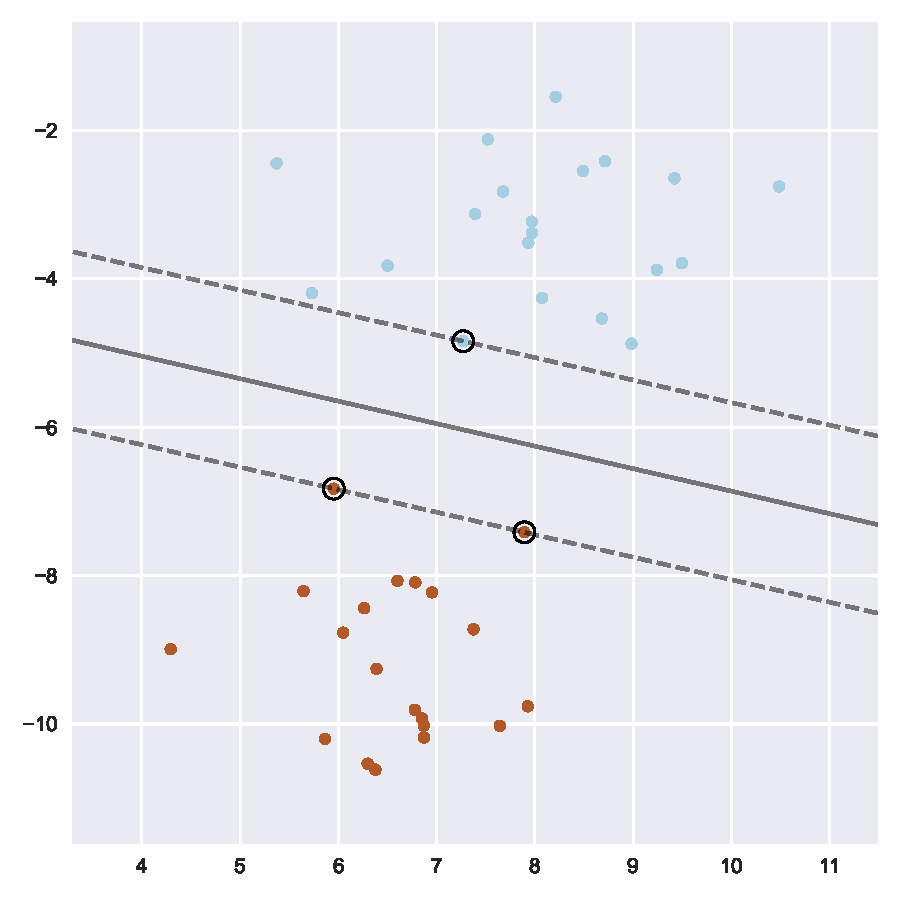
\includegraphics[width=14cm]{codeimage/code1}
	\caption{code1}
	\label{code1}
\end{figure}

\begin{PythonCode}\label{例2}
	\begin{Verbatim}[commandchars=\\\{\}]
\PY{c+c1}{\PYZsh{} 导入操作系统库}
\PY{k+kn}{import} \PY{n+nn}{os}
\PY{c+c1}{\PYZsh{} 更改工作目录}
\PY{n}{os}\PY{o}{.}\PY{n}{chdir}\PY{p}{(}\PY{l+s+sa}{r}\PY{l+s+s2}{\PYZdq{}}\PY{l+s+s2}{D:}\PY{l+s+s2}{\PYZbs{}}\PY{l+s+s2}{softwares}\PY{l+s+s2}{\PYZbs{}}\PY{l+s+s2}{applied statistics}\PY{l+s+s2}{\PYZbs{}}\PY{l+s+s2}{pythoncodelearning}\PY{l+s+s2}{\PYZbs{}}\PY{l+s+s2}{chap5}\PY{l+s+s2}{\PYZbs{}}\PY{l+s+s2}{sourcecode}\PY{l+s+s2}{\PYZdq{}}\PY{p}{)}
\PY{c+c1}{\PYZsh{} 导入绘图库}
\PY{k+kn}{import} \PY{n+nn}{matplotlib}\PY{n+nn}{.}\PY{n+nn}{pyplot} \PY{k}{as} \PY{n+nn}{plt}
\PY{c+c1}{\PYZsh{} 导入数据生成工具}
\PY{k+kn}{from} \PY{n+nn}{sklearn}\PY{n+nn}{.}\PY{n+nn}{datasets} \PY{k+kn}{import} \PY{n}{load\PYZus{}iris}
\PY{c+c1}{\PYZsh{} 导入决策树分类器}
\PY{k+kn}{from} \PY{n+nn}{sklearn}\PY{n+nn}{.}\PY{n+nn}{tree} \PY{k+kn}{import} \PY{n}{DecisionTreeClassifier}
\PY{c+c1}{\PYZsh{} 导入绘制树状图的工具}
\PY{k+kn}{from} \PY{n+nn}{sklearn}\PY{n+nn}{.}\PY{n+nn}{tree} \PY{k+kn}{import} \PY{n}{plot\PYZus{}tree}
\PY{c+c1}{\PYZsh{} 导入绘图库中的字体管理包}
\PY{k+kn}{from} \PY{n+nn}{matplotlib} \PY{k+kn}{import} \PY{n}{font\PYZus{}manager}
\PY{c+c1}{\PYZsh{} 实现中文字符正常显示}
\PY{n}{font} \PY{o}{=} \PY{n}{font\PYZus{}manager}\PY{o}{.}\PY{n}{FontProperties}\PY{p}{(}\PY{n}{fname}\PY{o}{=}\PY{l+s+sa}{r}\PY{l+s+s2}{\PYZdq{}}\PY{l+s+s2}{C:}\PY{l+s+s2}{\PYZbs{}}\PY{l+s+s2}{Windows}\PY{l+s+s2}{\PYZbs{}}\PY{l+s+s2}{Fonts}\PY{l+s+s2}{\PYZbs{}}\PY{l+s+s2}{SimKai.ttf}\PY{l+s+s2}{\PYZdq{}}\PY{p}{)}
\PY{c+c1}{\PYZsh{} 使用seaborn风格绘图}
\PY{n}{plt}\PY{o}{.}\PY{n}{style}\PY{o}{.}\PY{n}{use}\PY{p}{(}\PY{l+s+s2}{\PYZdq{}}\PY{l+s+s2}{seaborn\PYZhy{}v0\PYZus{}8}\PY{l+s+s2}{\PYZdq{}}\PY{p}{)}
\PY{c+c1}{\PYZsh{} 获取数据}
\PY{n}{iris} \PY{o}{=} \PY{n}{load\PYZus{}iris}\PY{p}{(}\PY{p}{)}
\PY{c+c1}{\PYZsh{} 构建模型}
\PY{n}{clf} \PY{o}{=} \PY{n}{DecisionTreeClassifier}\PY{p}{(}\PY{p}{)}
\PY{c+c1}{\PYZsh{} 模型拟合}
\PY{n}{clf}\PY{o}{.}\PY{n}{fit}\PY{p}{(}\PY{n}{iris}\PY{o}{.}\PY{n}{data}\PY{p}{,} \PY{n}{iris}\PY{o}{.}\PY{n}{target}\PY{p}{)}
\PY{n}{fig}\PY{p}{,} \PY{n}{ax} \PY{o}{=} \PY{n}{plt}\PY{o}{.}\PY{n}{subplots}\PY{p}{(}\PY{n}{figsize}\PY{o}{=}\PY{p}{(}\PY{l+m+mi}{6}\PY{p}{,}\PY{l+m+mi}{6}\PY{p}{)}\PY{p}{,} \PY{n}{tight\PYZus{}layout}\PY{o}{=}\PY{k+kc}{True}\PY{p}{)}
\PY{n}{plot\PYZus{}tree}\PY{p}{(}\PY{n}{clf}\PY{p}{,} \PY{n}{filled}\PY{o}{=}\PY{k+kc}{True}\PY{p}{)}
\PY{n}{ax}\PY{o}{.}\PY{n}{set\PYZus{}title}\PY{p}{(}\PY{l+s+s2}{\PYZdq{}}\PY{l+s+s2}{Decision tree trained on all the iris features}\PY{l+s+s2}{\PYZdq{}}\PY{p}{)}
\PY{n}{plt}\PY{o}{.}\PY{n}{show}\PY{p}{(}\PY{p}{)}
\PY{n}{fig}\PY{o}{.}\PY{n}{savefig}\PY{p}{(}\PY{l+s+s2}{\PYZdq{}}\PY{l+s+s2}{../codeimage/code2.pdf}\PY{l+s+s2}{\PYZdq{}}\PY{p}{)}
\end{Verbatim}

\end{PythonCode}

\begin{figure}[htbp]
	\centering
	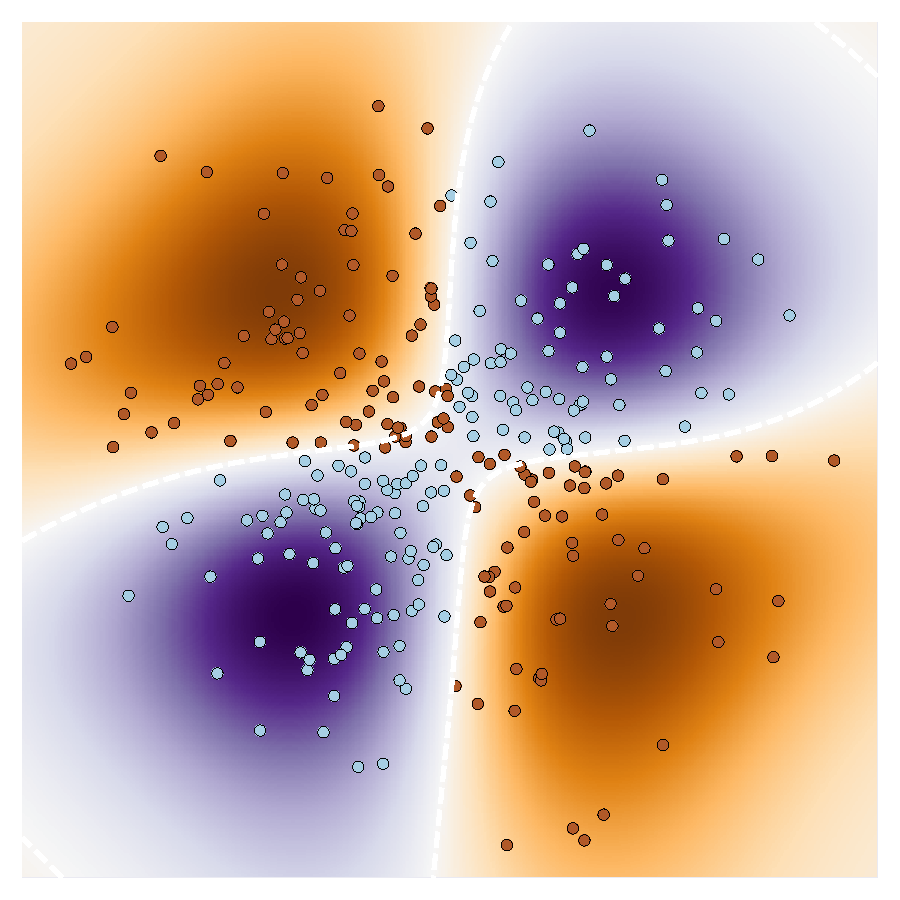
\includegraphics[width=14cm]{codeimage/code2}
	\caption{code2}
	\label{code2}
\end{figure}

\begin{PythonCode}\label{例3}
	\begin{Verbatim}[commandchars=\\\{\}]
\PY{c+c1}{\PYZsh{} 导入操作系统库}
\PY{k+kn}{import} \PY{n+nn}{os}
\PY{c+c1}{\PYZsh{} 更改工作目录}
\PY{n}{os}\PY{o}{.}\PY{n}{chdir}\PY{p}{(}\PY{l+s+sa}{r}\PY{l+s+s2}{\PYZdq{}}\PY{l+s+s2}{D:}\PY{l+s+s2}{\PYZbs{}}\PY{l+s+s2}{softwares}\PY{l+s+s2}{\PYZbs{}}\PY{l+s+s2}{applied statistics}\PY{l+s+s2}{\PYZbs{}}\PY{l+s+s2}{pythoncodelearning}\PY{l+s+s2}{\PYZbs{}}\PY{l+s+s2}{chap6}\PY{l+s+s2}{\PYZbs{}}\PY{l+s+s2}{sourcecode}\PY{l+s+s2}{\PYZdq{}}\PY{p}{)}
\PY{c+c1}{\PYZsh{} 导入基础计算库}
\PY{k+kn}{import} \PY{n+nn}{numpy} \PY{k}{as} \PY{n+nn}{np}
\PY{c+c1}{\PYZsh{} 导入绘图库}
\PY{k+kn}{import} \PY{n+nn}{matplotlib}\PY{n+nn}{.}\PY{n+nn}{pyplot} \PY{k}{as} \PY{n+nn}{plt}
\PY{c+c1}{\PYZsh{} 导入数据集工具}
\PY{k+kn}{from} \PY{n+nn}{sklearn}\PY{n+nn}{.}\PY{n+nn}{datasets} \PY{k+kn}{import} \PY{n}{load\PYZus{}diabetes}
\PY{c+c1}{\PYZsh{} 导入集成模型}
\PY{k+kn}{from} \PY{n+nn}{sklearn}\PY{n+nn}{.}\PY{n+nn}{ensemble} \PY{k+kn}{import} \PY{n}{GradientBoostingRegressor}
\PY{c+c1}{\PYZsh{} 导入均方误差工具}
\PY{k+kn}{from} \PY{n+nn}{sklearn}\PY{n+nn}{.}\PY{n+nn}{metrics} \PY{k+kn}{import} \PY{n}{mean\PYZus{}squared\PYZus{}error}
\PY{c+c1}{\PYZsh{} 导入数据集划分工具}
\PY{k+kn}{from} \PY{n+nn}{sklearn}\PY{n+nn}{.}\PY{n+nn}{model\PYZus{}selection} \PY{k+kn}{import} \PY{n}{train\PYZus{}test\PYZus{}split}
\PY{c+c1}{\PYZsh{} 导入绘图库中的字体管理包}
\PY{k+kn}{from} \PY{n+nn}{matplotlib} \PY{k+kn}{import} \PY{n}{font\PYZus{}manager}
\PY{c+c1}{\PYZsh{} 实现中文字符正常显示}
\PY{n}{font} \PY{o}{=} \PY{n}{font\PYZus{}manager}\PY{o}{.}\PY{n}{FontProperties}\PY{p}{(}\PY{n}{fname}\PY{o}{=}\PY{l+s+sa}{r}\PY{l+s+s2}{\PYZdq{}}\PY{l+s+s2}{C:}\PY{l+s+s2}{\PYZbs{}}\PY{l+s+s2}{Windows}\PY{l+s+s2}{\PYZbs{}}\PY{l+s+s2}{Fonts}\PY{l+s+s2}{\PYZbs{}}\PY{l+s+s2}{SimKai.ttf}\PY{l+s+s2}{\PYZdq{}}\PY{p}{)}
\PY{c+c1}{\PYZsh{} 使用seaborn风格绘图}
\PY{n}{plt}\PY{o}{.}\PY{n}{style}\PY{o}{.}\PY{n}{use}\PY{p}{(}\PY{l+s+s2}{\PYZdq{}}\PY{l+s+s2}{seaborn\PYZhy{}v0\PYZus{}8}\PY{l+s+s2}{\PYZdq{}}\PY{p}{)}
\PY{c+c1}{\PYZsh{} 加载数据集}
\PY{n}{diabetes} \PY{o}{=} \PY{n}{load\PYZus{}diabetes}\PY{p}{(}\PY{p}{)}
\PY{n}{X}\PY{p}{,} \PY{n}{y} \PY{o}{=} \PY{n}{diabetes}\PY{o}{.}\PY{n}{data}\PY{p}{,} \PY{n}{diabetes}\PY{o}{.}\PY{n}{target}
\PY{c+c1}{\PYZsh{} 划分数据集}
\PY{n}{X\PYZus{}train}\PY{p}{,} \PY{n}{X\PYZus{}test}\PY{p}{,} \PY{n}{y\PYZus{}train}\PY{p}{,} \PY{n}{y\PYZus{}test} \PY{o}{=} \PY{n}{train\PYZus{}test\PYZus{}split}\PY{p}{(}
    \PY{n}{X}\PY{p}{,} \PY{n}{y}\PY{p}{,} \PY{n}{test\PYZus{}size}\PY{o}{=}\PY{l+m+mf}{0.1}\PY{p}{,} \PY{n}{random\PYZus{}state}\PY{o}{=}\PY{l+m+mi}{13}
\PY{p}{)}
\PY{c+c1}{\PYZsh{} 设置一些参数}
\PY{n}{params} \PY{o}{=} \PY{p}{\PYZob{}}
    \PY{l+s+s2}{\PYZdq{}}\PY{l+s+s2}{n\PYZus{}estimators}\PY{l+s+s2}{\PYZdq{}}\PY{p}{:} \PY{l+m+mi}{500}\PY{p}{,}
    \PY{l+s+s2}{\PYZdq{}}\PY{l+s+s2}{max\PYZus{}depth}\PY{l+s+s2}{\PYZdq{}}\PY{p}{:} \PY{l+m+mi}{4}\PY{p}{,}
    \PY{l+s+s2}{\PYZdq{}}\PY{l+s+s2}{min\PYZus{}samples\PYZus{}split}\PY{l+s+s2}{\PYZdq{}}\PY{p}{:} \PY{l+m+mi}{5}\PY{p}{,}
    \PY{l+s+s2}{\PYZdq{}}\PY{l+s+s2}{learning\PYZus{}rate}\PY{l+s+s2}{\PYZdq{}}\PY{p}{:} \PY{l+m+mf}{0.01}\PY{p}{,}
    \PY{l+s+s2}{\PYZdq{}}\PY{l+s+s2}{loss}\PY{l+s+s2}{\PYZdq{}}\PY{p}{:} \PY{l+s+s2}{\PYZdq{}}\PY{l+s+s2}{squared\PYZus{}error}\PY{l+s+s2}{\PYZdq{}}\PY{p}{,}
\PY{p}{\PYZcb{}}
\PY{c+c1}{\PYZsh{} 构建模型}
\PY{n}{reg} \PY{o}{=} \PY{n}{GradientBoostingRegressor}\PY{p}{(}\PY{o}{*}\PY{o}{*}\PY{n}{params}\PY{p}{)}
\PY{c+c1}{\PYZsh{} 模型拟合}
\PY{n}{reg}\PY{o}{.}\PY{n}{fit}\PY{p}{(}\PY{n}{X\PYZus{}train}\PY{p}{,} \PY{n}{y\PYZus{}train}\PY{p}{)}
\PY{c+c1}{\PYZsh{} 预测}
\PY{n}{y\PYZus{}pred} \PY{o}{=} \PY{n}{reg}\PY{o}{.}\PY{n}{predict}\PY{p}{(}\PY{n}{X\PYZus{}test}\PY{p}{)}
\PY{c+c1}{\PYZsh{} 均方误差}
\PY{n}{mse} \PY{o}{=} \PY{n}{mean\PYZus{}squared\PYZus{}error}\PY{p}{(}\PY{n}{y\PYZus{}test}\PY{p}{,} \PY{n}{y\PYZus{}pred}\PY{p}{)}
\PY{n+nb}{print}\PY{p}{(}\PY{l+s+s2}{\PYZdq{}}\PY{l+s+s2}{The mean squared error (MSE) on test set: }\PY{l+s+si}{\PYZob{}:.4f\PYZcb{}}\PY{l+s+s2}{\PYZdq{}}\PY{o}{.}\PY{n}{format}\PY{p}{(}\PY{n}{mse}\PY{p}{)}\PY{p}{)}
\PY{c+c1}{\PYZsh{} 初始化测试集上的mse}
\PY{n}{test\PYZus{}score} \PY{o}{=} \PY{n}{np}\PY{o}{.}\PY{n}{zeros}\PY{p}{(}\PY{p}{(}\PY{n}{params}\PY{p}{[}\PY{l+s+s2}{\PYZdq{}}\PY{l+s+s2}{n\PYZus{}estimators}\PY{l+s+s2}{\PYZdq{}}\PY{p}{]}\PY{p}{,}\PY{p}{)}\PY{p}{,} \PY{n}{dtype}\PY{o}{=}\PY{n}{np}\PY{o}{.}\PY{n}{float64}\PY{p}{)}
\PY{c+c1}{\PYZsh{} 阶段性预测X\PYZus{}test}
\PY{k}{for} \PY{n}{i}\PY{p}{,} \PY{n}{y\PYZus{}pred} \PY{o+ow}{in} \PY{n+nb}{enumerate}\PY{p}{(}\PY{n}{reg}\PY{o}{.}\PY{n}{staged\PYZus{}predict}\PY{p}{(}\PY{n}{X\PYZus{}test}\PY{p}{)}\PY{p}{)}\PY{p}{:}
    \PY{c+c1}{\PYZsh{} 得到回归的mse}
    \PY{n}{test\PYZus{}score}\PY{p}{[}\PY{n}{i}\PY{p}{]} \PY{o}{=} \PY{n}{mean\PYZus{}squared\PYZus{}error}\PY{p}{(}\PY{n}{y\PYZus{}test}\PY{p}{,} \PY{n}{y\PYZus{}pred}\PY{p}{)}

\PY{n}{fig}\PY{p}{,} \PY{n}{ax} \PY{o}{=} \PY{n}{plt}\PY{o}{.}\PY{n}{subplots}\PY{p}{(}\PY{n}{figsize}\PY{o}{=}\PY{p}{(}\PY{l+m+mi}{6}\PY{p}{,} \PY{l+m+mi}{6}\PY{p}{)}\PY{p}{,} \PY{n}{tight\PYZus{}layout}\PY{o}{=}\PY{k+kc}{True}\PY{p}{)}
\PY{n}{ax}\PY{o}{.}\PY{n}{set\PYZus{}title}\PY{p}{(}\PY{l+s+s2}{\PYZdq{}}\PY{l+s+s2}{Deviance}\PY{l+s+s2}{\PYZdq{}}\PY{p}{)}
\PY{n}{ax}\PY{o}{.}\PY{n}{plot}\PY{p}{(}
    \PY{n}{np}\PY{o}{.}\PY{n}{arange}\PY{p}{(}\PY{n}{params}\PY{p}{[}\PY{l+s+s2}{\PYZdq{}}\PY{l+s+s2}{n\PYZus{}estimators}\PY{l+s+s2}{\PYZdq{}}\PY{p}{]}\PY{p}{)} \PY{o}{+} \PY{l+m+mi}{1}\PY{p}{,}
    \PY{n}{reg}\PY{o}{.}\PY{n}{train\PYZus{}score\PYZus{}}\PY{p}{,}
    \PY{l+s+s2}{\PYZdq{}}\PY{l+s+s2}{b\PYZhy{}}\PY{l+s+s2}{\PYZdq{}}\PY{p}{,}
    \PY{n}{label}\PY{o}{=}\PY{l+s+s2}{\PYZdq{}}\PY{l+s+s2}{Training Set Deviance}\PY{l+s+s2}{\PYZdq{}}\PY{p}{,}
\PY{p}{)}
\PY{n}{ax}\PY{o}{.}\PY{n}{plot}\PY{p}{(}
    \PY{n}{np}\PY{o}{.}\PY{n}{arange}\PY{p}{(}\PY{n}{params}\PY{p}{[}\PY{l+s+s2}{\PYZdq{}}\PY{l+s+s2}{n\PYZus{}estimators}\PY{l+s+s2}{\PYZdq{}}\PY{p}{]}\PY{p}{)} \PY{o}{+} \PY{l+m+mi}{1}\PY{p}{,} 
    \PY{n}{test\PYZus{}score}\PY{p}{,} \PY{l+s+s2}{\PYZdq{}}\PY{l+s+s2}{r\PYZhy{}}\PY{l+s+s2}{\PYZdq{}}\PY{p}{,} \PY{n}{label}\PY{o}{=}\PY{l+s+s2}{\PYZdq{}}\PY{l+s+s2}{Test Set Deviance}\PY{l+s+s2}{\PYZdq{}}
\PY{p}{)}
\PY{n}{ax}\PY{o}{.}\PY{n}{legend}\PY{p}{(}\PY{n}{loc}\PY{o}{=}\PY{l+s+s2}{\PYZdq{}}\PY{l+s+s2}{upper right}\PY{l+s+s2}{\PYZdq{}}\PY{p}{)}
\PY{n}{ax}\PY{o}{.}\PY{n}{set\PYZus{}xlabel}\PY{p}{(}\PY{l+s+s2}{\PYZdq{}}\PY{l+s+s2}{Boosting Iterations}\PY{l+s+s2}{\PYZdq{}}\PY{p}{)}
\PY{n}{ax}\PY{o}{.}\PY{n}{set\PYZus{}ylabel}\PY{p}{(}\PY{l+s+s2}{\PYZdq{}}\PY{l+s+s2}{Deviance}\PY{l+s+s2}{\PYZdq{}}\PY{p}{)}
\PY{n}{plt}\PY{o}{.}\PY{n}{show}\PY{p}{(}\PY{p}{)}
\PY{n}{fig}\PY{o}{.}\PY{n}{savefig}\PY{p}{(}\PY{l+s+s2}{\PYZdq{}}\PY{l+s+s2}{../codeimage/code3.pdf}\PY{l+s+s2}{\PYZdq{}}\PY{p}{)}
\end{Verbatim}

\begin{Verbatim}[commandchars=\\\{\}]
The mean squared error (MSE) on test set: 3041.0505
\end{Verbatim}
\end{PythonCode}

\begin{figure}[htbp]
	\centering
	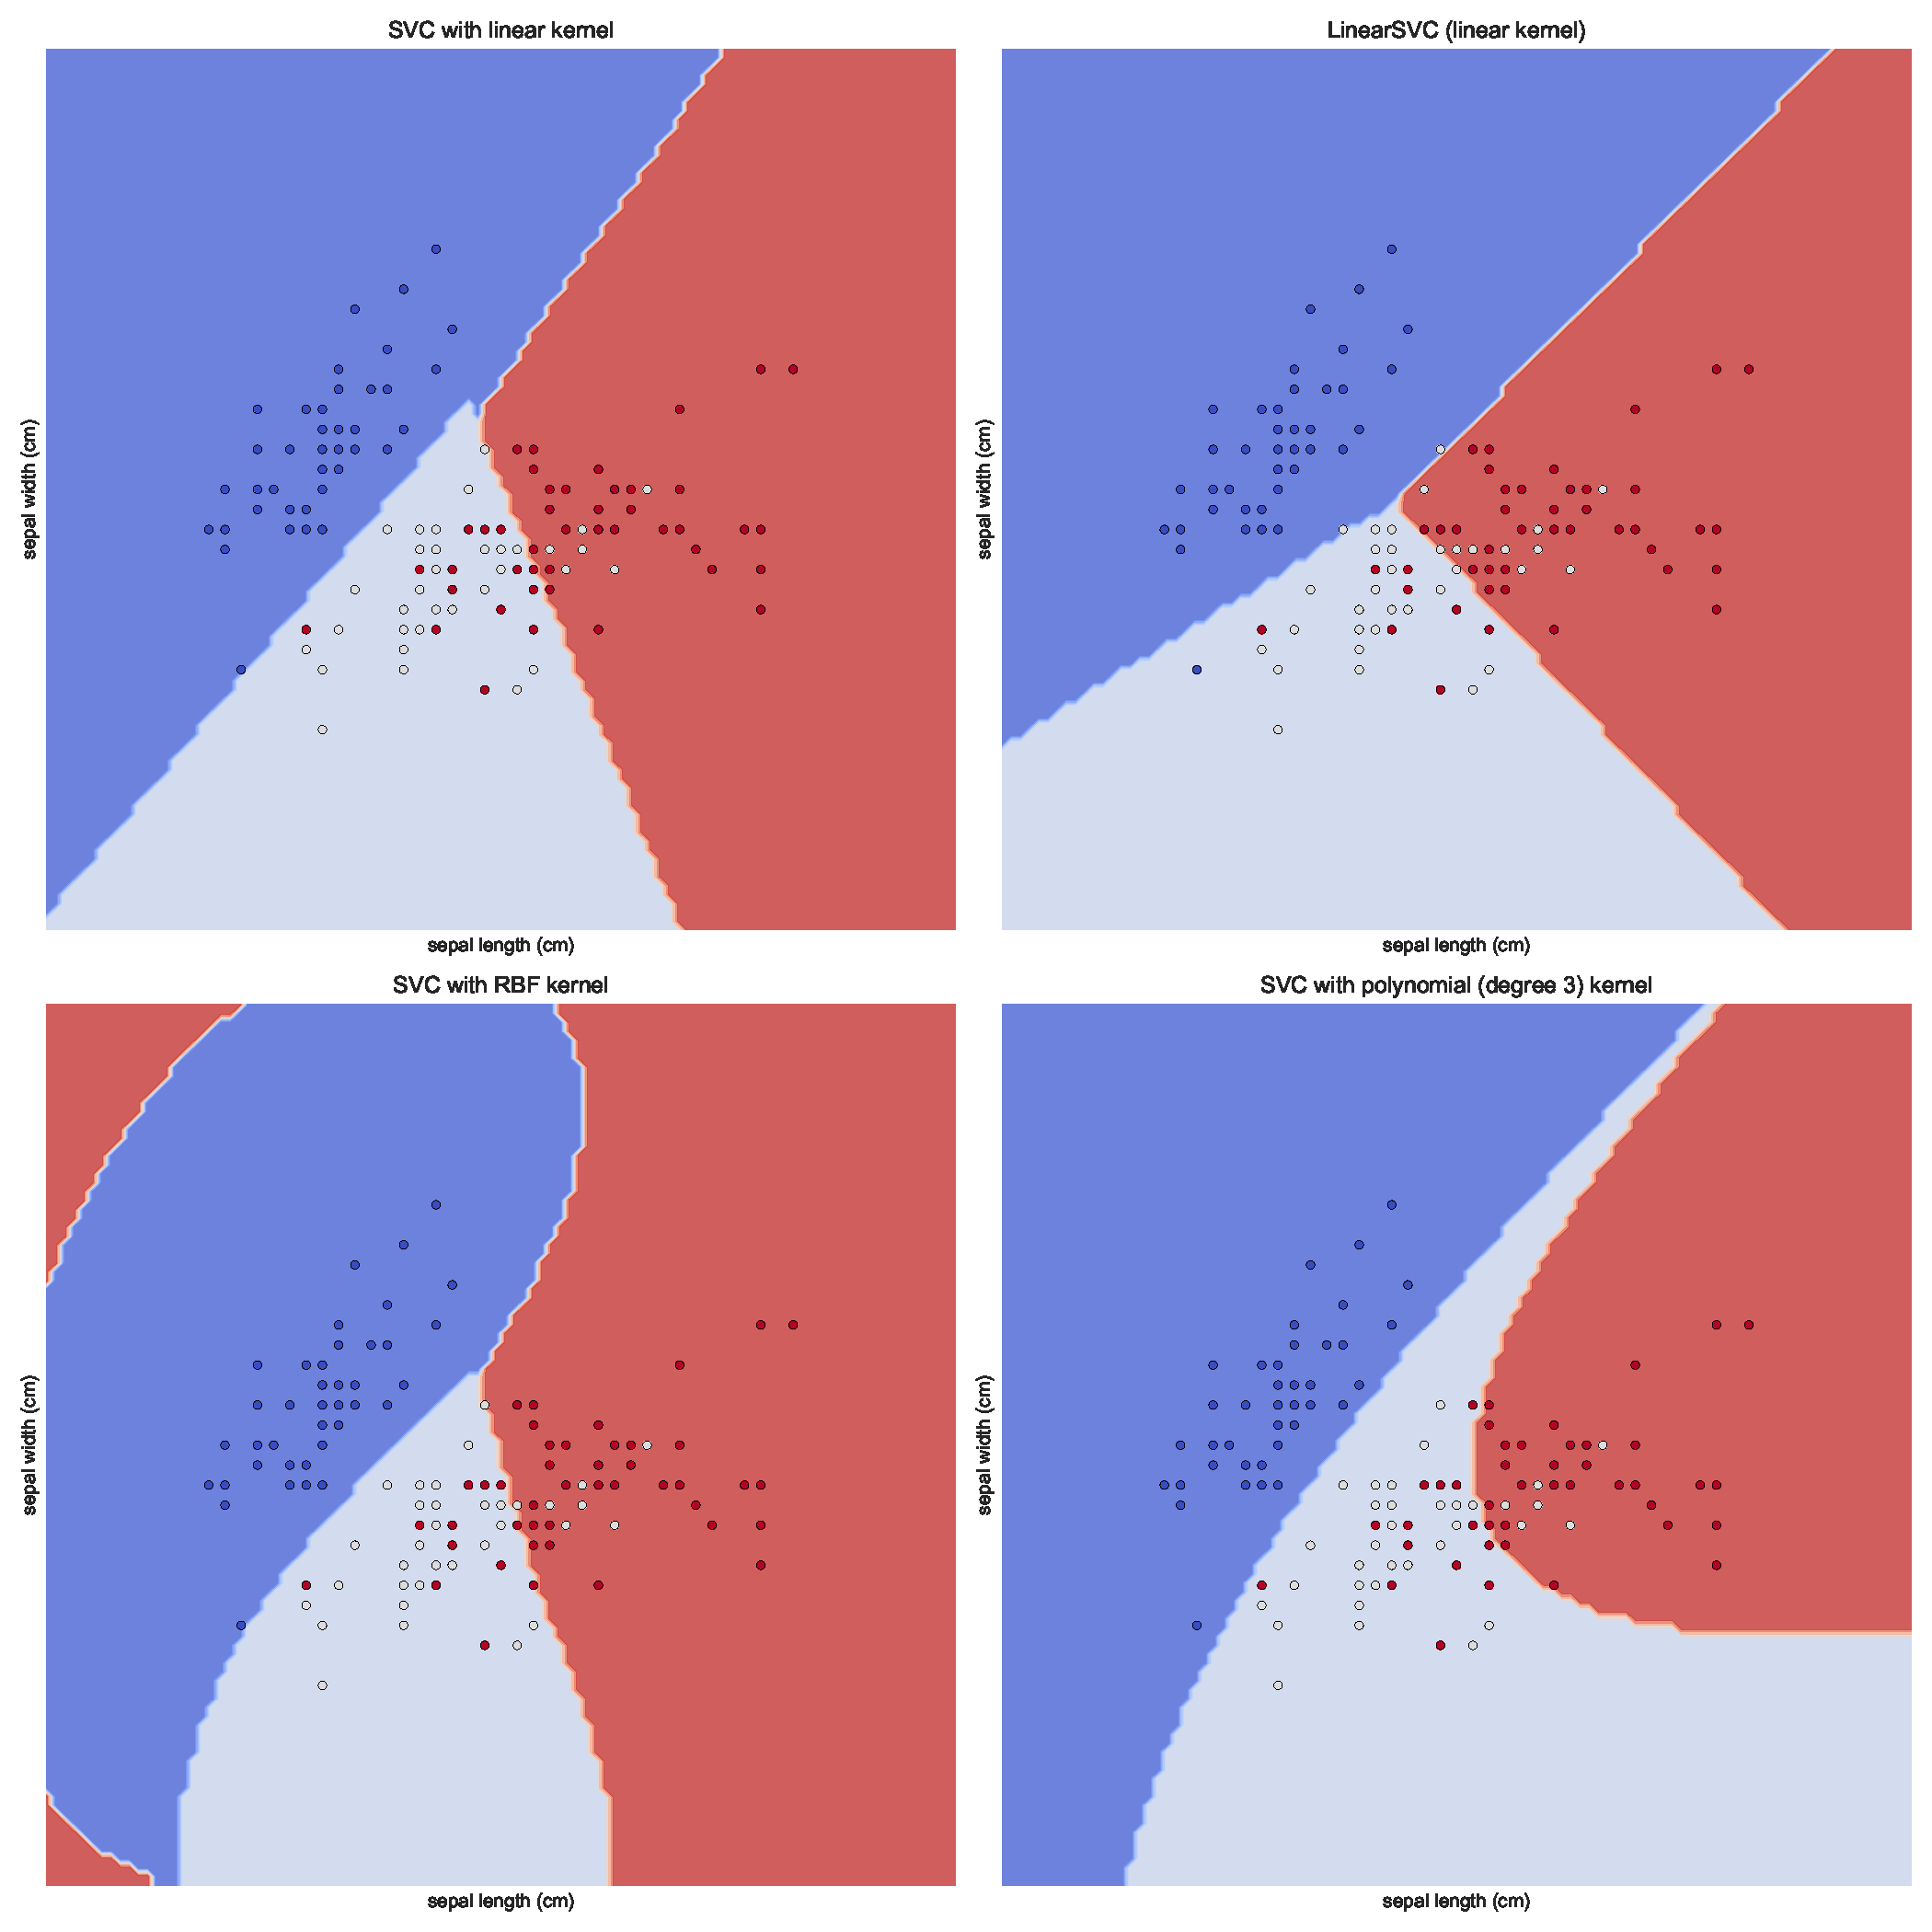
\includegraphics[width=14cm]{codeimage/code3}
	\caption{code3}
	\label{code3}
\end{figure}

\begin{PythonCode}\label{例4}
	\begin{Verbatim}[commandchars=\\\{\}]
\PY{c+c1}{\PYZsh{} 导入操作系统库}
\PY{k+kn}{import} \PY{n+nn}{os}
\PY{c+c1}{\PYZsh{} 更改工作目录}
\PY{n}{os}\PY{o}{.}\PY{n}{chdir}\PY{p}{(}\PY{l+s+sa}{r}\PY{l+s+s2}{\PYZdq{}}\PY{l+s+s2}{D:}\PY{l+s+s2}{\PYZbs{}}\PY{l+s+s2}{softwares}\PY{l+s+s2}{\PYZbs{}}\PY{l+s+s2}{applied statistics}\PY{l+s+s2}{\PYZbs{}}\PY{l+s+s2}{pythoncodelearning}\PY{l+s+s2}{\PYZbs{}}\PY{l+s+s2}{chap5}\PY{l+s+s2}{\PYZbs{}}\PY{l+s+s2}{sourcecode}\PY{l+s+s2}{\PYZdq{}}\PY{p}{)}
\PY{c+c1}{\PYZsh{} 导入绘图库}
\PY{k+kn}{import} \PY{n+nn}{matplotlib}\PY{n+nn}{.}\PY{n+nn}{pyplot} \PY{k}{as} \PY{n+nn}{plt}
\PY{c+c1}{\PYZsh{} 导入数据集划分工具}
\PY{k+kn}{from} \PY{n+nn}{sklearn}\PY{n+nn}{.}\PY{n+nn}{model\PYZus{}selection} \PY{k+kn}{import} \PY{n}{train\PYZus{}test\PYZus{}split}
\PY{c+c1}{\PYZsh{} 导入数据集工具}
\PY{k+kn}{from} \PY{n+nn}{sklearn}\PY{n+nn}{.}\PY{n+nn}{datasets} \PY{k+kn}{import} \PY{n}{load\PYZus{}breast\PYZus{}cancer}
\PY{c+c1}{\PYZsh{} 导入分类树}
\PY{k+kn}{from} \PY{n+nn}{sklearn}\PY{n+nn}{.}\PY{n+nn}{tree} \PY{k+kn}{import} \PY{n}{DecisionTreeClassifier}
\PY{c+c1}{\PYZsh{} 导入绘图库中的字体管理包}
\PY{k+kn}{from} \PY{n+nn}{matplotlib} \PY{k+kn}{import} \PY{n}{font\PYZus{}manager}
\PY{c+c1}{\PYZsh{} 实现中文字符正常显示}
\PY{n}{font} \PY{o}{=} \PY{n}{font\PYZus{}manager}\PY{o}{.}\PY{n}{FontProperties}\PY{p}{(}\PY{n}{fname}\PY{o}{=}\PY{l+s+sa}{r}\PY{l+s+s2}{\PYZdq{}}\PY{l+s+s2}{C:}\PY{l+s+s2}{\PYZbs{}}\PY{l+s+s2}{Windows}\PY{l+s+s2}{\PYZbs{}}\PY{l+s+s2}{Fonts}\PY{l+s+s2}{\PYZbs{}}\PY{l+s+s2}{SimKai.ttf}\PY{l+s+s2}{\PYZdq{}}\PY{p}{)}
\PY{c+c1}{\PYZsh{} 使用seaborn风格绘图}
\PY{n}{plt}\PY{o}{.}\PY{n}{style}\PY{o}{.}\PY{n}{use}\PY{p}{(}\PY{l+s+s2}{\PYZdq{}}\PY{l+s+s2}{seaborn\PYZhy{}v0\PYZus{}8}\PY{l+s+s2}{\PYZdq{}}\PY{p}{)}
\PY{c+c1}{\PYZsh{} 获取数据}
\PY{n}{X}\PY{p}{,} \PY{n}{y} \PY{o}{=} \PY{n}{load\PYZus{}breast\PYZus{}cancer}\PY{p}{(}\PY{n}{return\PYZus{}X\PYZus{}y}\PY{o}{=}\PY{k+kc}{True}\PY{p}{)}
\PY{c+c1}{\PYZsh{} 数据集划分}
\PY{n}{X\PYZus{}train}\PY{p}{,} \PY{n}{X\PYZus{}test}\PY{p}{,} \PY{n}{y\PYZus{}train}\PY{p}{,} \PY{n}{y\PYZus{}test} \PY{o}{=} \PY{n}{train\PYZus{}test\PYZus{}split}\PY{p}{(}
    \PY{n}{X}\PY{p}{,} \PY{n}{y}\PY{p}{,} \PY{n}{random\PYZus{}state}\PY{o}{=}\PY{l+m+mi}{0}
\PY{p}{)}
\PY{c+c1}{\PYZsh{} 构建决策树}
\PY{n}{clf} \PY{o}{=} \PY{n}{DecisionTreeClassifier}\PY{p}{(}\PY{n}{random\PYZus{}state}\PY{o}{=}\PY{l+m+mi}{0}\PY{p}{)}
\PY{c+c1}{\PYZsh{} 代价复杂度路径}
\PY{n}{path} \PY{o}{=} \PY{n}{clf}\PY{o}{.}\PY{n}{cost\PYZus{}complexity\PYZus{}pruning\PYZus{}path}\PY{p}{(}\PY{n}{X\PYZus{}train}\PY{p}{,} \PY{n}{y\PYZus{}train}\PY{p}{)}
\PY{c+c1}{\PYZsh{} cp}
\PY{n}{ccp\PYZus{}alphas}\PY{p}{,} \PY{n}{impurities} \PY{o}{=} \PY{n}{path}\PY{o}{.}\PY{n}{ccp\PYZus{}alphas}\PY{p}{,} \PY{n}{path}\PY{o}{.}\PY{n}{impurities}
\PY{c+c1}{\PYZsh{} 绘图}
\PY{n}{fig}\PY{p}{,} \PY{n}{ax} \PY{o}{=} \PY{n}{plt}\PY{o}{.}\PY{n}{subplots}\PY{p}{(}\PY{n}{figsize}\PY{o}{=}\PY{p}{(}\PY{l+m+mi}{6}\PY{p}{,}\PY{l+m+mi}{6}\PY{p}{)}\PY{p}{)}
\PY{n}{ax}\PY{o}{.}\PY{n}{plot}\PY{p}{(}\PY{n}{ccp\PYZus{}alphas}\PY{p}{[}\PY{p}{:}\PY{o}{\PYZhy{}}\PY{l+m+mi}{1}\PY{p}{]}\PY{p}{,} \PY{n}{impurities}\PY{p}{[}\PY{p}{:}\PY{o}{\PYZhy{}}\PY{l+m+mi}{1}\PY{p}{]}\PY{p}{,} \PY{n}{marker}\PY{o}{=}\PY{l+s+s2}{\PYZdq{}}\PY{l+s+s2}{o}\PY{l+s+s2}{\PYZdq{}}\PY{p}{,} \PY{n}{drawstyle}\PY{o}{=}\PY{l+s+s2}{\PYZdq{}}\PY{l+s+s2}{steps\PYZhy{}post}\PY{l+s+s2}{\PYZdq{}}\PY{p}{)}
\PY{n}{ax}\PY{o}{.}\PY{n}{set\PYZus{}xlabel}\PY{p}{(}\PY{l+s+s2}{\PYZdq{}}\PY{l+s+s2}{effective alpha}\PY{l+s+s2}{\PYZdq{}}\PY{p}{)}
\PY{n}{ax}\PY{o}{.}\PY{n}{set\PYZus{}ylabel}\PY{p}{(}\PY{l+s+s2}{\PYZdq{}}\PY{l+s+s2}{total impurity of leaves}\PY{l+s+s2}{\PYZdq{}}\PY{p}{)}
\PY{n}{ax}\PY{o}{.}\PY{n}{set\PYZus{}title}\PY{p}{(}\PY{l+s+s2}{\PYZdq{}}\PY{l+s+s2}{Total Impurity vs effective alpha for training set}\PY{l+s+s2}{\PYZdq{}}\PY{p}{)}
\PY{n}{plt}\PY{o}{.}\PY{n}{show}\PY{p}{(}\PY{p}{)}
\PY{n}{fig}\PY{o}{.}\PY{n}{savefig}\PY{p}{(}\PY{l+s+s2}{\PYZdq{}}\PY{l+s+s2}{../codeimage/code4.pdf}\PY{l+s+s2}{\PYZdq{}}\PY{p}{)}
\PY{c+c1}{\PYZsh{} 不同的alpha下构建决策树}
\PY{n}{clfs} \PY{o}{=} \PY{p}{[}\PY{p}{]}
\PY{k}{for} \PY{n}{ccp\PYZus{}alpha} \PY{o+ow}{in} \PY{n}{ccp\PYZus{}alphas}\PY{p}{:}
    \PY{c+c1}{\PYZsh{} 构建模型}
    \PY{n}{clf} \PY{o}{=} \PY{n}{DecisionTreeClassifier}\PY{p}{(}
        \PY{n}{random\PYZus{}state}\PY{o}{=}\PY{l+m+mi}{0}\PY{p}{,} \PY{n}{ccp\PYZus{}alpha}\PY{o}{=}\PY{n}{ccp\PYZus{}alpha}
    \PY{p}{)}
    \PY{c+c1}{\PYZsh{} 模拟拟合}
    \PY{n}{clf}\PY{o}{.}\PY{n}{fit}\PY{p}{(}\PY{n}{X\PYZus{}train}\PY{p}{,} \PY{n}{y\PYZus{}train}\PY{p}{)}
    \PY{c+c1}{\PYZsh{} 加入到列表中}
    \PY{n}{clfs}\PY{o}{.}\PY{n}{append}\PY{p}{(}\PY{n}{clf}\PY{p}{)}
\PY{n+nb}{print}\PY{p}{(}
    \PY{l+s+s2}{\PYZdq{}}\PY{l+s+s2}{Number of nodes in the last tree is: }\PY{l+s+si}{\PYZob{}\PYZcb{}}\PY{l+s+s2}{ with ccp\PYZus{}alpha: }\PY{l+s+si}{\PYZob{}\PYZcb{}}\PY{l+s+s2}{\PYZdq{}}\PY{o}{.}\PY{n}{format}\PY{p}{(}
        \PY{n}{clfs}\PY{p}{[}\PY{o}{\PYZhy{}}\PY{l+m+mi}{1}\PY{p}{]}\PY{o}{.}\PY{n}{tree\PYZus{}}\PY{o}{.}\PY{n}{node\PYZus{}count}\PY{p}{,} \PY{n}{ccp\PYZus{}alphas}\PY{p}{[}\PY{o}{\PYZhy{}}\PY{l+m+mi}{1}\PY{p}{]}
    \PY{p}{)}
\PY{p}{)}
\PY{c+c1}{\PYZsh{} 去掉最后一个}
\PY{n}{clfs} \PY{o}{=} \PY{n}{clfs}\PY{p}{[}\PY{p}{:}\PY{o}{\PYZhy{}}\PY{l+m+mi}{1}\PY{p}{]}
\PY{n}{ccp\PYZus{}alphas} \PY{o}{=} \PY{n}{ccp\PYZus{}alphas}\PY{p}{[}\PY{p}{:}\PY{o}{\PYZhy{}}\PY{l+m+mi}{1}\PY{p}{]}
\PY{c+c1}{\PYZsh{} 节点数量}
\PY{n}{node\PYZus{}counts} \PY{o}{=} \PY{p}{[}\PY{n}{clf}\PY{o}{.}\PY{n}{tree\PYZus{}}\PY{o}{.}\PY{n}{node\PYZus{}count} \PY{k}{for} \PY{n}{clf} \PY{o+ow}{in} \PY{n}{clfs}\PY{p}{]}
\PY{c+c1}{\PYZsh{} 深度}
\PY{n}{depth} \PY{o}{=} \PY{p}{[}\PY{n}{clf}\PY{o}{.}\PY{n}{tree\PYZus{}}\PY{o}{.}\PY{n}{max\PYZus{}depth} \PY{k}{for} \PY{n}{clf} \PY{o+ow}{in} \PY{n}{clfs}\PY{p}{]}
\PY{n}{fig}\PY{p}{,} \PY{n}{ax} \PY{o}{=} \PY{n}{plt}\PY{o}{.}\PY{n}{subplots}\PY{p}{(}\PY{l+m+mi}{2}\PY{p}{,} \PY{l+m+mi}{1}\PY{p}{,} \PY{n}{figsize}\PY{o}{=}\PY{p}{(}\PY{l+m+mi}{6}\PY{p}{,}\PY{l+m+mi}{6}\PY{p}{)}\PY{p}{,} \PY{n}{tight\PYZus{}layout}\PY{o}{=}\PY{k+kc}{True}\PY{p}{)}
\PY{n}{ax}\PY{p}{[}\PY{l+m+mi}{0}\PY{p}{]}\PY{o}{.}\PY{n}{plot}\PY{p}{(}\PY{n}{ccp\PYZus{}alphas}\PY{p}{,} \PY{n}{node\PYZus{}counts}\PY{p}{,} \PY{n}{marker}\PY{o}{=}\PY{l+s+s2}{\PYZdq{}}\PY{l+s+s2}{o}\PY{l+s+s2}{\PYZdq{}}\PY{p}{,} \PY{n}{drawstyle}\PY{o}{=}\PY{l+s+s2}{\PYZdq{}}\PY{l+s+s2}{steps\PYZhy{}post}\PY{l+s+s2}{\PYZdq{}}\PY{p}{)}
\PY{n}{ax}\PY{p}{[}\PY{l+m+mi}{0}\PY{p}{]}\PY{o}{.}\PY{n}{set\PYZus{}xlabel}\PY{p}{(}\PY{l+s+s2}{\PYZdq{}}\PY{l+s+s2}{alpha}\PY{l+s+s2}{\PYZdq{}}\PY{p}{)}
\PY{n}{ax}\PY{p}{[}\PY{l+m+mi}{0}\PY{p}{]}\PY{o}{.}\PY{n}{set\PYZus{}ylabel}\PY{p}{(}\PY{l+s+s2}{\PYZdq{}}\PY{l+s+s2}{number of nodes}\PY{l+s+s2}{\PYZdq{}}\PY{p}{)}
\PY{n}{ax}\PY{p}{[}\PY{l+m+mi}{0}\PY{p}{]}\PY{o}{.}\PY{n}{set\PYZus{}title}\PY{p}{(}\PY{l+s+s2}{\PYZdq{}}\PY{l+s+s2}{Number of nodes vs alpha}\PY{l+s+s2}{\PYZdq{}}\PY{p}{)}
\PY{n}{ax}\PY{p}{[}\PY{l+m+mi}{1}\PY{p}{]}\PY{o}{.}\PY{n}{plot}\PY{p}{(}\PY{n}{ccp\PYZus{}alphas}\PY{p}{,} \PY{n}{depth}\PY{p}{,} \PY{n}{marker}\PY{o}{=}\PY{l+s+s2}{\PYZdq{}}\PY{l+s+s2}{o}\PY{l+s+s2}{\PYZdq{}}\PY{p}{,} \PY{n}{drawstyle}\PY{o}{=}\PY{l+s+s2}{\PYZdq{}}\PY{l+s+s2}{steps\PYZhy{}post}\PY{l+s+s2}{\PYZdq{}}\PY{p}{)}
\PY{n}{ax}\PY{p}{[}\PY{l+m+mi}{1}\PY{p}{]}\PY{o}{.}\PY{n}{set\PYZus{}xlabel}\PY{p}{(}\PY{l+s+s2}{\PYZdq{}}\PY{l+s+s2}{alpha}\PY{l+s+s2}{\PYZdq{}}\PY{p}{)}
\PY{n}{ax}\PY{p}{[}\PY{l+m+mi}{1}\PY{p}{]}\PY{o}{.}\PY{n}{set\PYZus{}ylabel}\PY{p}{(}\PY{l+s+s2}{\PYZdq{}}\PY{l+s+s2}{depth of tree}\PY{l+s+s2}{\PYZdq{}}\PY{p}{)}
\PY{n}{ax}\PY{p}{[}\PY{l+m+mi}{1}\PY{p}{]}\PY{o}{.}\PY{n}{set\PYZus{}title}\PY{p}{(}\PY{l+s+s2}{\PYZdq{}}\PY{l+s+s2}{Depth vs alpha}\PY{l+s+s2}{\PYZdq{}}\PY{p}{)}
\PY{n}{plt}\PY{o}{.}\PY{n}{show}\PY{p}{(}\PY{p}{)}
\PY{n}{fig}\PY{o}{.}\PY{n}{savefig}\PY{p}{(}\PY{l+s+s2}{\PYZdq{}}\PY{l+s+s2}{../codeimage/code5.pdf}\PY{l+s+s2}{\PYZdq{}}\PY{p}{)}
\PY{c+c1}{\PYZsh{} 预测精度和alpha的关系}
\PY{c+c1}{\PYZsh{} 训练集的准确率}
\PY{n}{train\PYZus{}scores} \PY{o}{=} \PY{p}{[}\PY{n}{clf}\PY{o}{.}\PY{n}{score}\PY{p}{(}\PY{n}{X\PYZus{}train}\PY{p}{,} \PY{n}{y\PYZus{}train}\PY{p}{)} \PY{k}{for} \PY{n}{clf} \PY{o+ow}{in} \PY{n}{clfs}\PY{p}{]}
\PY{c+c1}{\PYZsh{} 测试集的准确率}
\PY{n}{test\PYZus{}scores} \PY{o}{=} \PY{p}{[}\PY{n}{clf}\PY{o}{.}\PY{n}{score}\PY{p}{(}\PY{n}{X\PYZus{}test}\PY{p}{,} \PY{n}{y\PYZus{}test}\PY{p}{)} \PY{k}{for} \PY{n}{clf} \PY{o+ow}{in} \PY{n}{clfs}\PY{p}{]}
\PY{n}{fig}\PY{p}{,} \PY{n}{ax} \PY{o}{=} \PY{n}{plt}\PY{o}{.}\PY{n}{subplots}\PY{p}{(}\PY{n}{figsize}\PY{o}{=}\PY{p}{(}\PY{l+m+mi}{6}\PY{p}{,}\PY{l+m+mi}{6}\PY{p}{)}\PY{p}{)}
\PY{n}{ax}\PY{o}{.}\PY{n}{set\PYZus{}xlabel}\PY{p}{(}\PY{l+s+s2}{\PYZdq{}}\PY{l+s+s2}{alpha}\PY{l+s+s2}{\PYZdq{}}\PY{p}{)}
\PY{n}{ax}\PY{o}{.}\PY{n}{set\PYZus{}ylabel}\PY{p}{(}\PY{l+s+s2}{\PYZdq{}}\PY{l+s+s2}{accuracy}\PY{l+s+s2}{\PYZdq{}}\PY{p}{)}
\PY{n}{ax}\PY{o}{.}\PY{n}{set\PYZus{}title}\PY{p}{(}\PY{l+s+s2}{\PYZdq{}}\PY{l+s+s2}{Accuracy vs alpha for training and testing sets}\PY{l+s+s2}{\PYZdq{}}\PY{p}{)}
\PY{n}{ax}\PY{o}{.}\PY{n}{plot}\PY{p}{(}\PY{n}{ccp\PYZus{}alphas}\PY{p}{,} \PY{n}{train\PYZus{}scores}\PY{p}{,} \PY{n}{marker}\PY{o}{=}\PY{l+s+s2}{\PYZdq{}}\PY{l+s+s2}{o}\PY{l+s+s2}{\PYZdq{}}\PY{p}{,} \PY{n}{label}\PY{o}{=}\PY{l+s+s2}{\PYZdq{}}\PY{l+s+s2}{train}\PY{l+s+s2}{\PYZdq{}}\PY{p}{,} \PY{n}{drawstyle}\PY{o}{=}\PY{l+s+s2}{\PYZdq{}}\PY{l+s+s2}{steps\PYZhy{}post}\PY{l+s+s2}{\PYZdq{}}\PY{p}{)}
\PY{n}{ax}\PY{o}{.}\PY{n}{plot}\PY{p}{(}\PY{n}{ccp\PYZus{}alphas}\PY{p}{,} \PY{n}{test\PYZus{}scores}\PY{p}{,} \PY{n}{marker}\PY{o}{=}\PY{l+s+s2}{\PYZdq{}}\PY{l+s+s2}{o}\PY{l+s+s2}{\PYZdq{}}\PY{p}{,} \PY{n}{label}\PY{o}{=}\PY{l+s+s2}{\PYZdq{}}\PY{l+s+s2}{test}\PY{l+s+s2}{\PYZdq{}}\PY{p}{,} \PY{n}{drawstyle}\PY{o}{=}\PY{l+s+s2}{\PYZdq{}}\PY{l+s+s2}{steps\PYZhy{}post}\PY{l+s+s2}{\PYZdq{}}\PY{p}{)}
\PY{n}{ax}\PY{o}{.}\PY{n}{legend}\PY{p}{(}\PY{p}{)}
\PY{n}{plt}\PY{o}{.}\PY{n}{show}\PY{p}{(}\PY{p}{)}
\PY{n}{fig}\PY{o}{.}\PY{n}{savefig}\PY{p}{(}\PY{l+s+s2}{\PYZdq{}}\PY{l+s+s2}{../codeimage/code6.pdf}\PY{l+s+s2}{\PYZdq{}}\PY{p}{)}
\end{Verbatim}
    
\begin{Verbatim}[commandchars=\\\{\}]
Number of nodes in the last tree is: 1 with ccp\_alpha: 0.3272984419327777
\end{Verbatim}
\end{PythonCode}

\begin{figure}[htbp]
	\centering
	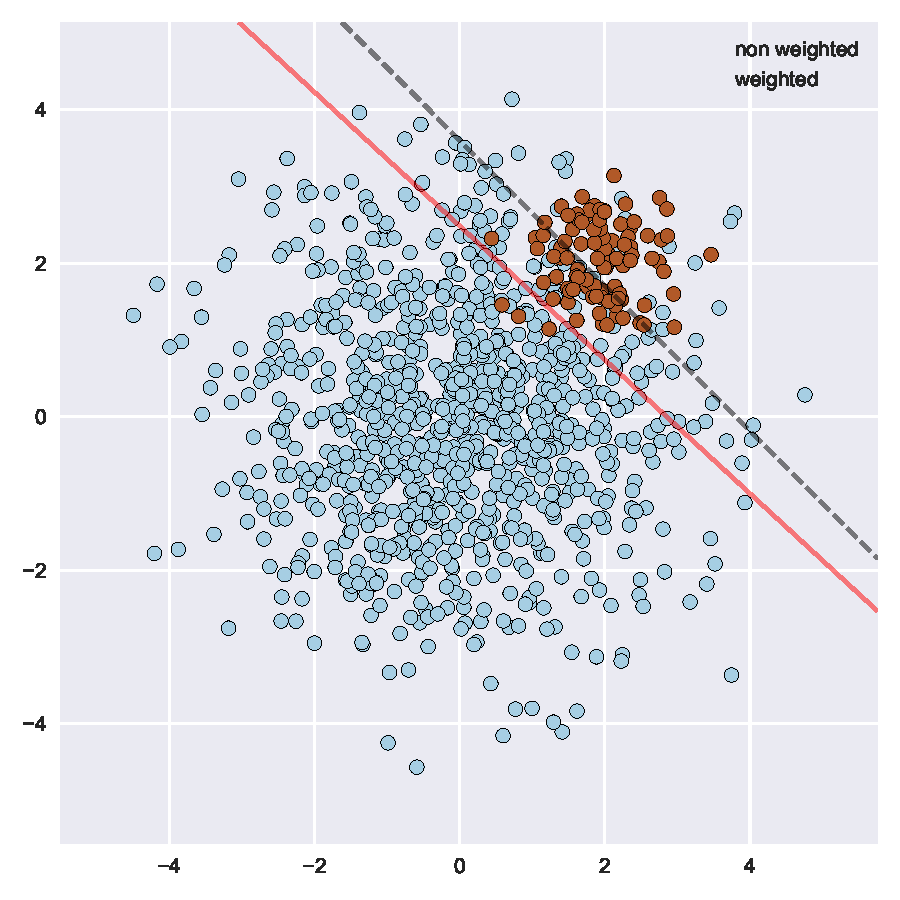
\includegraphics[width=14cm]{codeimage/code4}
	\caption{code4}
	\label{code4}
\end{figure}

\begin{PythonCode}\label{例5}
	\begin{Verbatim}[commandchars=\\\{\}]
\PY{c+c1}{\PYZsh{} 导入操作系统库}
\PY{k+kn}{import} \PY{n+nn}{os}
\PY{c+c1}{\PYZsh{} 更改工作目录}
\PY{n}{os}\PY{o}{.}\PY{n}{chdir}\PY{p}{(}\PY{l+s+sa}{r}\PY{l+s+s2}{\PYZdq{}}\PY{l+s+s2}{D:}\PY{l+s+s2}{\PYZbs{}}\PY{l+s+s2}{softwares}\PY{l+s+s2}{\PYZbs{}}\PY{l+s+s2}{applied statistics}\PY{l+s+s2}{\PYZbs{}}\PY{l+s+s2}{pythoncodelearning}\PY{l+s+s2}{\PYZbs{}}\PY{l+s+s2}{chap3}\PY{l+s+s2}{\PYZbs{}}\PY{l+s+s2}{sourcecode}\PY{l+s+s2}{\PYZdq{}}\PY{p}{)}
\PY{c+c1}{\PYZsh{} 导入基础计算库}
\PY{k+kn}{import} \PY{n+nn}{numpy} \PY{k}{as} \PY{n+nn}{np}
\PY{c+c1}{\PYZsh{} 导入绘图库}
\PY{k+kn}{import} \PY{n+nn}{matplotlib}\PY{n+nn}{.}\PY{n+nn}{pyplot} \PY{k}{as} \PY{n+nn}{plt}
\PY{c+c1}{\PYZsh{} 导入支持向量机模型}
\PY{k+kn}{from} \PY{n+nn}{sklearn}\PY{n+nn}{.}\PY{n+nn}{svm} \PY{k+kn}{import} \PY{n}{SVR}
\PY{c+c1}{\PYZsh{} 导入绘图库中的字体管理包}
\PY{k+kn}{from} \PY{n+nn}{matplotlib} \PY{k+kn}{import} \PY{n}{font\PYZus{}manager}
\PY{c+c1}{\PYZsh{} 实现中文字符正常显示}
\PY{n}{font} \PY{o}{=} \PY{n}{font\PYZus{}manager}\PY{o}{.}\PY{n}{FontProperties}\PY{p}{(}\PY{n}{fname}\PY{o}{=}\PY{l+s+sa}{r}\PY{l+s+s2}{\PYZdq{}}\PY{l+s+s2}{C:}\PY{l+s+s2}{\PYZbs{}}\PY{l+s+s2}{Windows}\PY{l+s+s2}{\PYZbs{}}\PY{l+s+s2}{Fonts}\PY{l+s+s2}{\PYZbs{}}\PY{l+s+s2}{SimKai.ttf}\PY{l+s+s2}{\PYZdq{}}\PY{p}{)}
\PY{c+c1}{\PYZsh{} 使用seaborn风格绘图}
\PY{n}{plt}\PY{o}{.}\PY{n}{style}\PY{o}{.}\PY{n}{use}\PY{p}{(}\PY{l+s+s2}{\PYZdq{}}\PY{l+s+s2}{seaborn\PYZhy{}v0\PYZus{}8}\PY{l+s+s2}{\PYZdq{}}\PY{p}{)}
\PY{c+c1}{\PYZsh{} 生成样本}
\PY{n}{X} \PY{o}{=} \PY{n}{np}\PY{o}{.}\PY{n}{sort}\PY{p}{(}\PY{l+m+mi}{5} \PY{o}{*} \PY{n}{np}\PY{o}{.}\PY{n}{random}\PY{o}{.}\PY{n}{rand}\PY{p}{(}\PY{l+m+mi}{40}\PY{p}{,} \PY{l+m+mi}{1}\PY{p}{)}\PY{p}{,} \PY{n}{axis}\PY{o}{=}\PY{l+m+mi}{0}\PY{p}{)}
\PY{n}{y} \PY{o}{=} \PY{n}{np}\PY{o}{.}\PY{n}{sin}\PY{p}{(}\PY{n}{X}\PY{p}{)}\PY{o}{.}\PY{n}{ravel}\PY{p}{(}\PY{p}{)}
\PY{c+c1}{\PYZsh{} 添加噪声}
\PY{n}{y}\PY{p}{[}\PY{p}{:}\PY{p}{:}\PY{l+m+mi}{5}\PY{p}{]} \PY{o}{+}\PY{o}{=} \PY{l+m+mi}{3} \PY{o}{*} \PY{p}{(}\PY{l+m+mf}{0.5} \PY{o}{\PYZhy{}} \PY{n}{np}\PY{o}{.}\PY{n}{random}\PY{o}{.}\PY{n}{rand}\PY{p}{(}\PY{l+m+mi}{8}\PY{p}{)}\PY{p}{)}
\PY{c+c1}{\PYZsh{} rbf核函数的SVR}
\PY{n}{svr\PYZus{}rbf} \PY{o}{=} \PY{n}{SVR}\PY{p}{(}\PY{n}{kernel}\PY{o}{=}\PY{l+s+s2}{\PYZdq{}}\PY{l+s+s2}{rbf}\PY{l+s+s2}{\PYZdq{}}\PY{p}{,} \PY{n}{C}\PY{o}{=}\PY{l+m+mi}{100}\PY{p}{,} \PY{n}{gamma}\PY{o}{=}\PY{l+m+mf}{0.1}\PY{p}{,} \PY{n}{epsilon}\PY{o}{=}\PY{l+m+mf}{0.1}\PY{p}{)}
\PY{c+c1}{\PYZsh{} 线性核函数的SVR}
\PY{n}{svr\PYZus{}lin} \PY{o}{=} \PY{n}{SVR}\PY{p}{(}\PY{n}{kernel}\PY{o}{=}\PY{l+s+s2}{\PYZdq{}}\PY{l+s+s2}{linear}\PY{l+s+s2}{\PYZdq{}}\PY{p}{,} \PY{n}{C}\PY{o}{=}\PY{l+m+mi}{100}\PY{p}{,} \PY{n}{gamma}\PY{o}{=}\PY{l+s+s2}{\PYZdq{}}\PY{l+s+s2}{auto}\PY{l+s+s2}{\PYZdq{}}\PY{p}{)}
\PY{c+c1}{\PYZsh{} 多项式核函数的SVR}
\PY{n}{svr\PYZus{}poly} \PY{o}{=} \PY{n}{SVR}\PY{p}{(}\PY{n}{kernel}\PY{o}{=}\PY{l+s+s2}{\PYZdq{}}\PY{l+s+s2}{poly}\PY{l+s+s2}{\PYZdq{}}\PY{p}{,} \PY{n}{C}\PY{o}{=}\PY{l+m+mi}{100}\PY{p}{,} \PY{n}{gamma}\PY{o}{=}\PY{l+s+s2}{\PYZdq{}}\PY{l+s+s2}{auto}\PY{l+s+s2}{\PYZdq{}}\PY{p}{,} \PY{n}{degree}\PY{o}{=}\PY{l+m+mi}{3}\PY{p}{,} \PY{n}{epsilon}\PY{o}{=}\PY{l+m+mf}{0.1}\PY{p}{,} \PY{n}{coef0}\PY{o}{=}\PY{l+m+mi}{1}\PY{p}{)}
\PY{n}{lw} \PY{o}{=} \PY{l+m+mi}{2}
\PY{c+c1}{\PYZsh{} 构造迭代对象列表}
\PY{n}{svrs} \PY{o}{=} \PY{p}{[}\PY{n}{svr\PYZus{}rbf}\PY{p}{,} \PY{n}{svr\PYZus{}lin}\PY{p}{,} \PY{n}{svr\PYZus{}poly}\PY{p}{]}
\PY{n}{kernel\PYZus{}label} \PY{o}{=} \PY{p}{[}\PY{l+s+s2}{\PYZdq{}}\PY{l+s+s2}{RBF}\PY{l+s+s2}{\PYZdq{}}\PY{p}{,} \PY{l+s+s2}{\PYZdq{}}\PY{l+s+s2}{Linear}\PY{l+s+s2}{\PYZdq{}}\PY{p}{,} \PY{l+s+s2}{\PYZdq{}}\PY{l+s+s2}{Polynomial}\PY{l+s+s2}{\PYZdq{}}\PY{p}{]}
\PY{n}{model\PYZus{}color} \PY{o}{=} \PY{p}{[}\PY{l+s+s2}{\PYZdq{}}\PY{l+s+s2}{m}\PY{l+s+s2}{\PYZdq{}}\PY{p}{,} \PY{l+s+s2}{\PYZdq{}}\PY{l+s+s2}{c}\PY{l+s+s2}{\PYZdq{}}\PY{p}{,} \PY{l+s+s2}{\PYZdq{}}\PY{l+s+s2}{g}\PY{l+s+s2}{\PYZdq{}}\PY{p}{]}
\PY{c+c1}{\PYZsh{} 开始绘图}
\PY{n}{fig}\PY{p}{,} \PY{n}{axes} \PY{o}{=} \PY{n}{plt}\PY{o}{.}\PY{n}{subplots}\PY{p}{(}\PY{n}{nrows}\PY{o}{=}\PY{l+m+mi}{1}\PY{p}{,} \PY{n}{ncols}\PY{o}{=}\PY{l+m+mi}{3}\PY{p}{,} \PY{n}{figsize}\PY{o}{=}\PY{p}{(}\PY{l+m+mi}{15}\PY{p}{,} \PY{l+m+mi}{10}\PY{p}{)}\PY{p}{,} \PY{n}{sharey}\PY{o}{=}\PY{k+kc}{True}\PY{p}{)}
\PY{k}{for} \PY{n}{ix}\PY{p}{,} \PY{n}{svr} \PY{o+ow}{in} \PY{n+nb}{enumerate}\PY{p}{(}\PY{n}{svrs}\PY{p}{)}\PY{p}{:}
    \PY{n}{axes}\PY{p}{[}\PY{n}{ix}\PY{p}{]}\PY{o}{.}\PY{n}{plot}\PY{p}{(}
        \PY{n}{X}\PY{p}{,}
        \PY{n}{svr}\PY{o}{.}\PY{n}{fit}\PY{p}{(}\PY{n}{X}\PY{p}{,} \PY{n}{y}\PY{p}{)}\PY{o}{.}\PY{n}{predict}\PY{p}{(}\PY{n}{X}\PY{p}{)}\PY{p}{,}
        \PY{n}{color}\PY{o}{=}\PY{n}{model\PYZus{}color}\PY{p}{[}\PY{n}{ix}\PY{p}{]}\PY{p}{,}
        \PY{n}{lw}\PY{o}{=}\PY{n}{lw}\PY{p}{,}
        \PY{n}{label}\PY{o}{=}\PY{l+s+s2}{\PYZdq{}}\PY{l+s+si}{\PYZob{}\PYZcb{}}\PY{l+s+s2}{ model}\PY{l+s+s2}{\PYZdq{}}\PY{o}{.}\PY{n}{format}\PY{p}{(}\PY{n}{kernel\PYZus{}label}\PY{p}{[}\PY{n}{ix}\PY{p}{]}\PY{p}{)}\PY{p}{,}
    \PY{p}{)}
    \PY{n}{axes}\PY{p}{[}\PY{n}{ix}\PY{p}{]}\PY{o}{.}\PY{n}{scatter}\PY{p}{(}
        \PY{n}{X}\PY{p}{[}\PY{n}{svr}\PY{o}{.}\PY{n}{support\PYZus{}}\PY{p}{]}\PY{p}{,}
        \PY{n}{y}\PY{p}{[}\PY{n}{svr}\PY{o}{.}\PY{n}{support\PYZus{}}\PY{p}{]}\PY{p}{,}
        \PY{n}{facecolor}\PY{o}{=}\PY{l+s+s2}{\PYZdq{}}\PY{l+s+s2}{none}\PY{l+s+s2}{\PYZdq{}}\PY{p}{,}
        \PY{n}{edgecolor}\PY{o}{=}\PY{n}{model\PYZus{}color}\PY{p}{[}\PY{n}{ix}\PY{p}{]}\PY{p}{,}
        \PY{n}{s}\PY{o}{=}\PY{l+m+mi}{50}\PY{p}{,}
        \PY{n}{label}\PY{o}{=}\PY{l+s+s2}{\PYZdq{}}\PY{l+s+si}{\PYZob{}\PYZcb{}}\PY{l+s+s2}{ support vectors}\PY{l+s+s2}{\PYZdq{}}\PY{o}{.}\PY{n}{format}\PY{p}{(}\PY{n}{kernel\PYZus{}label}\PY{p}{[}\PY{n}{ix}\PY{p}{]}\PY{p}{)}\PY{p}{,}
    \PY{p}{)}
    \PY{n}{axes}\PY{p}{[}\PY{n}{ix}\PY{p}{]}\PY{o}{.}\PY{n}{scatter}\PY{p}{(}
        \PY{n}{X}\PY{p}{[}\PY{n}{np}\PY{o}{.}\PY{n}{setdiff1d}\PY{p}{(}\PY{n}{np}\PY{o}{.}\PY{n}{arange}\PY{p}{(}\PY{n+nb}{len}\PY{p}{(}\PY{n}{X}\PY{p}{)}\PY{p}{)}\PY{p}{,} \PY{n}{svr}\PY{o}{.}\PY{n}{support\PYZus{}}\PY{p}{)}\PY{p}{]}\PY{p}{,}
        \PY{n}{y}\PY{p}{[}\PY{n}{np}\PY{o}{.}\PY{n}{setdiff1d}\PY{p}{(}\PY{n}{np}\PY{o}{.}\PY{n}{arange}\PY{p}{(}\PY{n+nb}{len}\PY{p}{(}\PY{n}{X}\PY{p}{)}\PY{p}{)}\PY{p}{,} \PY{n}{svr}\PY{o}{.}\PY{n}{support\PYZus{}}\PY{p}{)}\PY{p}{]}\PY{p}{,}
        \PY{n}{facecolor}\PY{o}{=}\PY{l+s+s2}{\PYZdq{}}\PY{l+s+s2}{none}\PY{l+s+s2}{\PYZdq{}}\PY{p}{,}
        \PY{n}{edgecolor}\PY{o}{=}\PY{l+s+s2}{\PYZdq{}}\PY{l+s+s2}{k}\PY{l+s+s2}{\PYZdq{}}\PY{p}{,}
        \PY{n}{s}\PY{o}{=}\PY{l+m+mi}{50}\PY{p}{,}
        \PY{n}{label}\PY{o}{=}\PY{l+s+s2}{\PYZdq{}}\PY{l+s+s2}{other training data}\PY{l+s+s2}{\PYZdq{}}\PY{p}{,}
    \PY{p}{)}
    \PY{n}{axes}\PY{p}{[}\PY{n}{ix}\PY{p}{]}\PY{o}{.}\PY{n}{legend}\PY{p}{(}
        \PY{n}{loc}\PY{o}{=}\PY{l+s+s2}{\PYZdq{}}\PY{l+s+s2}{upper center}\PY{l+s+s2}{\PYZdq{}}\PY{p}{,}
        \PY{n}{bbox\PYZus{}to\PYZus{}anchor}\PY{o}{=}\PY{p}{(}\PY{l+m+mf}{0.5}\PY{p}{,} \PY{l+m+mf}{1.1}\PY{p}{)}\PY{p}{,}
        \PY{n}{ncol}\PY{o}{=}\PY{l+m+mi}{1}\PY{p}{,}
        \PY{n}{fancybox}\PY{o}{=}\PY{k+kc}{True}\PY{p}{,}
        \PY{n}{shadow}\PY{o}{=}\PY{k+kc}{True}\PY{p}{,}
    \PY{p}{)}

\PY{n}{fig}\PY{o}{.}\PY{n}{text}\PY{p}{(}\PY{l+m+mf}{0.5}\PY{p}{,} \PY{l+m+mf}{0.04}\PY{p}{,} \PY{l+s+s2}{\PYZdq{}}\PY{l+s+s2}{data}\PY{l+s+s2}{\PYZdq{}}\PY{p}{,} \PY{n}{ha}\PY{o}{=}\PY{l+s+s2}{\PYZdq{}}\PY{l+s+s2}{center}\PY{l+s+s2}{\PYZdq{}}\PY{p}{,} \PY{n}{va}\PY{o}{=}\PY{l+s+s2}{\PYZdq{}}\PY{l+s+s2}{center}\PY{l+s+s2}{\PYZdq{}}\PY{p}{)}
\PY{n}{fig}\PY{o}{.}\PY{n}{text}\PY{p}{(}\PY{l+m+mf}{0.06}\PY{p}{,} \PY{l+m+mf}{0.5}\PY{p}{,} \PY{l+s+s2}{\PYZdq{}}\PY{l+s+s2}{target}\PY{l+s+s2}{\PYZdq{}}\PY{p}{,} \PY{n}{ha}\PY{o}{=}\PY{l+s+s2}{\PYZdq{}}\PY{l+s+s2}{center}\PY{l+s+s2}{\PYZdq{}}\PY{p}{,} \PY{n}{va}\PY{o}{=}\PY{l+s+s2}{\PYZdq{}}\PY{l+s+s2}{center}\PY{l+s+s2}{\PYZdq{}}\PY{p}{,} \PY{n}{rotation}\PY{o}{=}\PY{l+s+s2}{\PYZdq{}}\PY{l+s+s2}{vertical}\PY{l+s+s2}{\PYZdq{}}\PY{p}{)}
\PY{n}{fig}\PY{o}{.}\PY{n}{suptitle}\PY{p}{(}\PY{l+s+s2}{\PYZdq{}}\PY{l+s+s2}{Support Vector Regression}\PY{l+s+s2}{\PYZdq{}}\PY{p}{,} \PY{n}{fontsize}\PY{o}{=}\PY{l+m+mi}{14}\PY{p}{)}
\PY{n}{plt}\PY{o}{.}\PY{n}{show}\PY{p}{(}\PY{p}{)}
\PY{n}{fig}\PY{o}{.}\PY{n}{savefig}\PY{p}{(}\PY{l+s+s2}{\PYZdq{}}\PY{l+s+s2}{../codeimage/code5.pdf}\PY{l+s+s2}{\PYZdq{}}\PY{p}{)}
\end{Verbatim}

\end{PythonCode}

\begin{figure}[htbp]
	\centering
	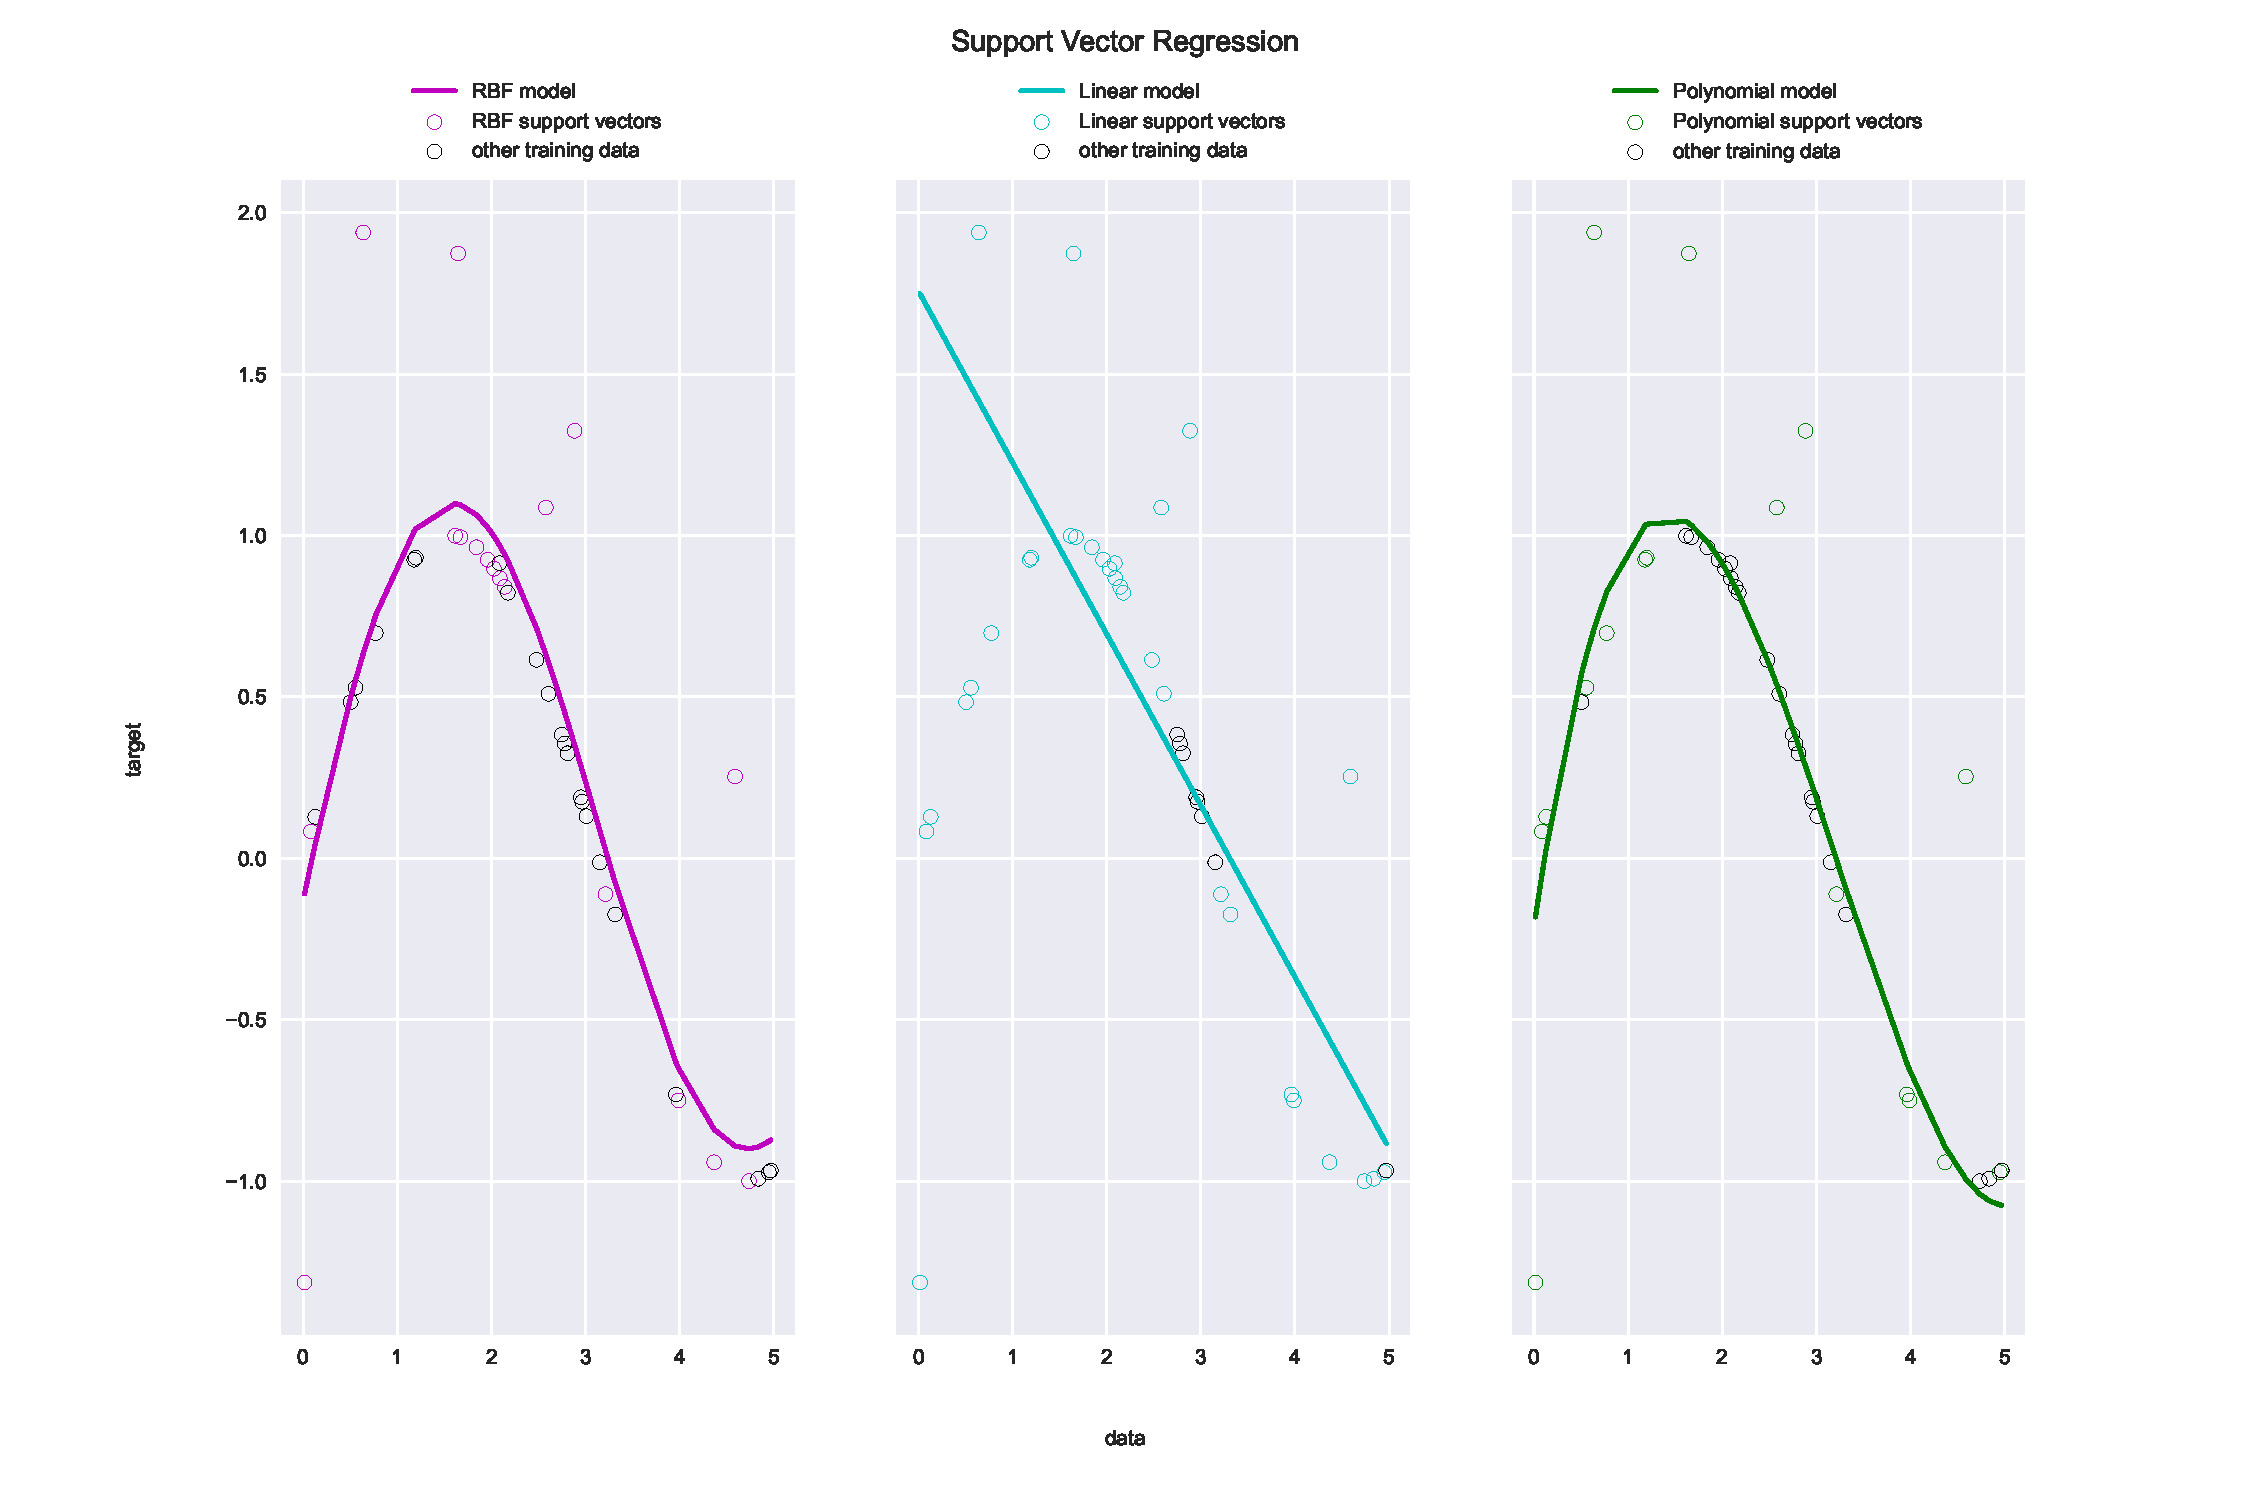
\includegraphics[width=14cm]{codeimage/code5}
	\caption{code5}
	\label{code5}
\end{figure}
